\documentclass[a4paper,12pt]{article}%
\usepackage{amsfonts}
\usepackage{amssymb}
\usepackage{amsmath}
\usepackage{eurosym}
\usepackage{latexsym}
\usepackage{graphicx}
\usepackage{longtable}
\usepackage{portland}
\usepackage{lscape}
\usepackage[onehalfspacing]{setspace}
\usepackage{footmisc}
\usepackage{fancyhdr}
\usepackage{hyphenat}
\usepackage{rotating}
\usepackage[USenglish]{babel}
\usepackage{array}
\usepackage{tabularx}
\usepackage{chicago}
\usepackage{theorem}
\usepackage{epstopdf}
\usepackage{makeidx}
\usepackage[left=1in,right=1in,top=1in,bottom=1in]{geometry}
\setcounter{MaxMatrixCols}{30}
\newtheorem{theorem}{Theorem}
\newtheorem{acknowledgement}[theorem]{Acknowledgement}
\newtheorem{algorithm}[theorem]{Algorithm}
\newtheorem{assum}{Assumption}
\newtheorem{axiom}[theorem]{Axiom}
\newtheorem{case}[theorem]{Case}
\newtheorem{claim}[theorem]{Claim}
\newtheorem{conclusion}[theorem]{Conclusion}
\newtheorem{condition}[theorem]{Condition}
\newtheorem{conjecture}[theorem]{Conjecture}
\newtheorem{corollary}[theorem]{Corollary}
\newtheorem{criterion}[theorem]{Criterion}
\newtheorem{definition}{Definition}
\newtheorem{example}[theorem]{Example}
\newtheorem{exercise}[theorem]{Exercise}
\newtheorem{lemma}[theorem]{Lemma}
\newtheorem{notation}[theorem]{Notation}
\newtheorem{problem}[theorem]{Problem}
\newtheorem{proposition}{Proposition}
\newtheorem{remark}[theorem]{Remark}
\newtheorem{solution}[theorem]{Solution}
\newtheorem{summary}[theorem]{Summary}
\newtheorem{observation}{Observation}
\newtheorem{result}{Result}

\newcolumntype{L}[1]{>{\raggedright\arraybackslash}p{#1}} % linksbündig mit Breitenangabe
\newcolumntype{C}[1]{>{\centering\arraybackslash}p{#1}} % zentriert mit Breitenangabe
\newcolumntype{R}[1]{>{\raggedleft\arraybackslash}p{#1}} % rechtsbündig mit Breitenangabe

\begin{document}

\title{Endogenous Grids in Higher Dimensions: Delaunay Interpolation and Hybrid Methods\thanks{We thank Johannes Brumm, Christopher Carroll, Michael Reiter and seminar participants at University of Cologne, the 2012 CEF and the Cologne Macroeconomic Workshop 2012 for helpful comments.}}
\author{Alexander Ludwig\thanks{CMR \& FiFo, University of Cologne; MEA; Netspar; Albertus-Magnus-Platz; 50923 K\"oln; Germany; E-mail: ludwig@wiso.uni-koeln.de}
\and Matthias Sch\"{o}n\thanks{CMR, University of Cologne; Albertus-Magnus-Platz; 50923 K\"{o}ln; Germany; E-mail: m.schoen@wiso.uni-koeln.de}}
\date{\today }
\maketitle

\begin{abstract}
This paper investigates extensions of the method of endogenous grid-points (ENDGM) introduced by Carroll (2006) to higher dimensions with more than one continuous endogenous state variable. We compare three different categories ofalgorithms: (i) the conventional method with exogenous grids (EXGM), (ii) the pure method of endogenous grid-points (ENDGM) and (iii) a hybrid method (HEGM). ENDGM comes along with Delaunay interpolation on irregular grids. Comparison of methods is done by evaluating speed and accuracy. We find that HEGM and ENDGM both dominate EXGM. The choice between HEGM and ENDGM depends on the number of dimensions and the number of grid-points in each dimension. With less than~150 grid-points in each dimension ENDGM is faster than HEGM, and vice versa. For a standard choice of~$20$ to~$40$ grid-points in each dimension, ENDGM is~$1.6$ to~$1.8$ times faster than HEGM. 
\newline\textit{JEL Classification: C63, E21.
\newline Keywords: Dynamic Models, Numerical Solution, Endogenous Gridpoints Method, Delaunay Interpolation}

\end{abstract}

\newpage\pagenumbering{arabic} \renewcommand{\thefootnote}{\arabic{footnote}} \setcounter{footnote}{0}

\section{Introduction}

Dynamic models of equilibrium in discrete time are workhorse models in Economics. However, most of these models do not have an analytic closed form solution and equilibria have to be approximated numerically. Numerous procedures have been developed in the literature, cf.~\citeN{judd98},~\citeN{miranda04}. If the problem is differentiable, a popular approach is to use first-order methods, i.e., to iterate on first-order conditions. An important contribution in this literature is~\citeN{carroll06} who introduces the method of endogenous grid points (ENDGM). In comparison to the method of exogenous grid-points (EXGM), ENDGM greatly enhances computational speed because part of the problem can be computed in closed form.

This paper investigates extensions of Carroll's method to dynamic problems with more than one continuous endogenous state variable. We highlight an important drawback of ENDGM in higher dimensions which is due to the endogenously computed states. The resulting state grid is not rectangular, i.e., grid-points are irregularly distributed in the space. In consequence, even linear interpolation is much more costly than for conventional rectangular grids. Hence, there exists a fundamental trade-off between EXGM and ENDGM in higher dimensions. On the one hand, EXGM requires the use of numerical routines throughout whereas ENDGM computes solutions to first-order conditions in closed form. On the other hand, interpolation in EXGM is on regular grids and therefore simple. Interpolation in ENDGM on irregular grids is much more complex. We solve this complex interpolation by Delaunay triangulation. Delaunay interpolation originally coming from the field of geometry is not commonly adopted in Economics. It was only recently introduced to the field by~\citeN{brumm10}.

In addition to EXGM and ENDGM, we consider a third algorithm, a hybrid method of exogenous and endogenous grid-points (HEGM). HEGM uses endogenous grids in some but not all dimensions. The trade-off between HEGM and ENDGM is therefore between costly routines in some dimensions vis-\`{a}-vis analytical solutions in all dimensions but a more complex interpolation.

To analyze and to compare these methods we use a simple human capital model. This model features two endogenous state variables, financial assets and human capital. Evaluation of methods in this two dimensional setup is done by comparing speed and accuracy of the different approaches.

Our main finding is that HEGM and ENDGM both dominate EXGM. They are both substantially faster. The choice between HEGM and ENDGM depends on the number of grid-points in each dimension. For a relatively low number of grid-points, ENDGM is advantageous and vice versa for HEGM. We discuss limitations of ENDGM and HEGM which are both only applicable for specific problems at hand. Furthermore, we argue that the relative advantage of HEGM decreases in higher dimensions (higher than two).

To the best of our knowledge ENDGM in higher dimensions is not yet fully understood. Our paper is an important contribution to fill this gap. Related work by~\citeN{krueger07} and~\citeN{Barillas07} extends ENDGM to problems with two control variables but just one endogenous state variable. \citeN{Hintermaier10} incorporate two endogenous state variables in a durable goods model and apply a version of HEGM. Their algorithm exploits the fact that durable goods consumption is zero at the end of life. In a human capital model such as ours this is not possible because the human capital stock is neither zero nor known at the end of life. Hence our version of HEGM differs from the \citeN{Hintermaier10} approach.

Our analysis proceeds as follows. Section~2 presents the simple human capital setting on which we base the evaluation of methods. Section~3 introduces the main features of the methods under evaluation, the method of exogenous grid-points, the pure method of endogenous grid-points and the hybrid method of exogenous and endogenous grid-points. Section~4 presents results according to speed and accuracy of all three methods. Section~5 concludes. Additional material is contained in an appendix.

\section{General Framework}

We develop a human capital model which allows us to illustrate and compare three approaches to solve dynamic models with two endogenous states using first-order methods. In addition to financial assets there is another endogenous state, a human or health capital stock (we will use both interpretations interchangeably). Human capital can be accumulated over time and is produced with a nonlinear production function. For expositional purposes we keep the model simple. Of course, the underlying trade-off between solution methods will also hold in more complex problems.

\subsection{A Simple Human Capital Model}

\label{ss:simplehkmodel}

We consider a setup in which the only risk is the risk to survive to the next period. A risk averse agent with maximum time horizon $T$, $T=\infty$ possible, derives utility from consumption, $c_{t},$ in each period, with standard additive separable life time utility
\[
U=\sum_{t=1}^{T}\beta^{t-1}s\left( h_{t} \right)  u\left( c_{t}\right),
\]
where $\beta\in\left( 0,1\right)$ is the discount factor. The instantaneous utility function~$u\left( c_{t}\right)$ is assumed to be strictly concave, and the probability to survive to the next period $s\left( h_{t}\right)$ is assumed to be non-linear in the accumulated human (or health) capital stock $h_{t}$. Income of the agent, $y_{t}$, consists of labor income which depends on the amount of accumulated human capital $h_{t}$,
\[
y_{t}=wh_{t},
\]
where $w$ is the wage rate.

In each period the household faces the decision to consume $c_{t}$, to invest in a risk-free financial asset, $a_{t}$, which earns (gross) interest $R$ and to invest an amount $i_{t}$ in human capital, $h_{t}$. Human capital depreciates at constant rate~$\delta$ and is produced by the production function $f\left( i\right)$. We assume that $f_{i}>0$, $f_{ii}<0$ and that the Inada conditions are satisfied, i.e., $\lim_{i_{t}\rightarrow0}f_{i}=\infty$ and~$\lim_{i_{t}\rightarrow\infty}f_{i}=0$. These conditions are crucial because otherwise it could turn out to be optimal to invest in only one asset. The other asset would be redundant and our problem would collapse to a problem in one dimension. The human capital accumulation equation is
accordingly given by
\begin{equation}
h_{t+1}=(1-\delta)\left( h_{t}+f\left( i_{t}\right) \right),
\label{eq:hkaccum}
\end{equation}
where $h_{0}$ is given.

Financial markets are imperfect and households are not allowed to hold negative financial assets. The budget constraint writes as
\[
a_{t+1} = R(a_{t} + w h_{t} - c_{t} - i_{t}) \geq0.
\]

\paragraph{Recursive Formulation of the Household Problem}

The recursive formulation of the household problem is as follows:
\[
V_{t}(a_{t},h_{t})=\underset{c_{t},i_{t},a_{t+1},h_{t+1}}{\max}\left\{u(c_{t})+\beta s\left(  h_{t+1}\right)  V_{t+1}(a_{t+1},h_{t+1})\right\}
\]
subject to the constraints
\begin{align}
a_{t+1}  &  =R\left(  a_{t}+wh_{t}-c_{t}-i_{t}\right) \nonumber\\
h_{t+1}  &  =\left(  1-\delta\right)  \left(  h_{t}+f\left(  i_{t}\right)\right) \nonumber\\
a_{t+1}  &  \geq0\nonumber\\
h_{t+1}  &  >0. \label{eq:hinequ}
\end{align}

\paragraph{Assumptions on Functional Forms}

For our numerical approach we assume that instantaneous utility has the CRRA property with coefficient of relative risk aversion denoted by~$\theta$:
\[
u\left( c_{t}\right) =\frac{c_{t}^{1-\theta}-1}{1-\theta}.
\]

The human capital production function is
\[
f\left( i_{t}\right) =\gamma\frac{i_{t}^{1-\alpha}-1}{1-\alpha}
\]
for curvature parameter~$\alpha>0$. As to the functional form of the per-period survival probability we follow~\citeN{hall07} and assume that
\[
s\left( h_{t}\right) = 1-\phi\frac{1}{1+h_{t}}\text{.}
\]

We assume that the value function is strictly concave and unique maximizers are continuous policy functions, cf.~\citeN{stokey89}. It is well-known that these conditions may not hold in human capital models because endogenous human capital formation may lead to non-convexities (value functions may have concave and convex regions). Hence, first-order conditions are generally necessary but not sufficient. In applications, one way to accommodate this is to use methods developed in this paper at the calibration stage of the model (where speed is an issue). Upon convergence, one can then test for uniqueness by checking for alternative solutions by use of global methods. To focus our analysis we do not further address these aspects here.

\paragraph{Solution}

The optimal solution is fully characterized by the following set of first-order conditions and constraints:
\begin{subequations}
\label{eq:eqsyst}
\begin{align}
c_{t}^{-\theta}  &  = \beta R \left[ 1-\phi\frac{1}{1+h_{t+1}}\right] \text{$V_{t+1_{a}}$}\left( a_{t+1},h_{t+1}\right) \label{Foc1} \\
i_{t}^{-\alpha}  &  = \frac{R}{\left( 1-\delta\right)} \frac{\text{$V_{t+1_{a}}$}\left( a_{t+1},h_{t+1}\right)}{\frac{\phi}{\left[1+h_{t+1}-\phi\right]  \left[ 1+h_{t+1}\right]}V_{t+1}\left(a_{t+1},h_{t+1}\right) +\text{$V_{t+1_{h}}$}\left( a_{t+1},h_{t+1}\right)} \label{Foc2} \\
a_{t+1}  &  = R \left( a_{t}+wh_{t}-c_{t}-i_{t}\right) \\
h_{t+1}  &  = \left( 1-\delta\right) \left( h_{t}+f\left( i_{t}\right)\right) \\
a_{t+1}  &  \geq0.
\end{align}
\end{subequations}
$V_{t_{a}}$ and $V_{t_{h}}$ are derivatives of the value function with respect to financial assets and human capital, respectively. The first equation relates today's consumption to consumption of tomorrow, whereas the second equation relates costs and gains of investing in human capital. Notice that constraint~(\ref{eq:hinequ}) can be dropped because of the lower Inada condition of the human capital investment function~$f(i)$. Searching for the solution of this model amounts to finding the four optimal policies for consumption, $c_{t}\left( \cdot,\cdot\right)$, investment in human capital, $i_{t}\left( \cdot,\cdot\right)$, next period's financial assets, $a_{t+1}\left( \cdot,\cdot\right)$, and next period's human capital, $h_{t+1}\left(  \cdot,\cdot\right)$, as functions of the two endogenous state variables, financial assets, $a_{t}$, and human capital, $h_{t}$, that solve equation system~(\ref{eq:eqsyst}).

The envelope conditions are:
\begin{subequations}
\begin{align}
\text{$V_{t_{a}}$}\left( a_{t},h_{t}\right)  &  =u_{c}=c_{t}^{-\theta} \label{Envelope1}\\
\text{$V_{t_{h}}$}\left( a_{t},h_{t}\right)  &  =\left( w+\frac{1}{f_{i}}\right) u_{c}=\left( w+\frac{1}{i_{t}^{-\alpha}}\right) c_{t}^{-\theta}\text{.} \label{Envelope2}
\end{align}
\end{subequations}
Using (\ref{Foc1}) together with (\ref{Envelope1}) gives the standard Euler equation of consumption.\footnote{For derivation of~(\ref{eq:eqsyst}) and the Envelope conditions see Appendix~A.}

\subsection{Calibration}

We choose the same parameterization of the model for all solution methods described in section~\ref{s:solmeth}. The coefficient of relative risk aversion parameter is set to $\theta=0.5$ to assure a positive value of life. We set the time preference rate to $\rho=0.04$. In order to achieve incentives to save in the finite horizon setting without introducing uncertainty we set an interest rate of $R-1=0.05$. In the infinite horizon setting we set an interest rate of $R-1=0.035$ smaller than $\rho$ to assure that financial assets are bounded. For the depreciation rate of human capital we take $\delta=0.05.$ The parameters of the human capital production function are $\alpha=0.65$ and $\gamma=1.0$, respectively. The wage rate $w$ is set to $0.1$. The survival rate parameter is $\phi=0.5$.

\section{Solution Methods}
\label{s:solmeth}

The main idea of all methods is to exploit the FOCs~(\ref{Foc1}) and~(\ref{Foc2}) to compute optimal policies at discrete points that constitute a mesh in the state space. All three methods use the recursive nature of the problem. Correspondingly, in the finite horizon version the model is solved backwards from the last to the first period ($t=T,...,0$). In the infinite horizon implementation the iteration continues until convergence on policy functions.

Differences between methods arise because of different solution procedures to the multi-dimensional nonlinear equation system~(\ref{eq:eqsyst}) and different interpolation methods, respectively. The first algorithm (EXGM) applies a multi-dimensional Quasi-Newton method. Standard interpolation methods are used. The second algorithm (ENDGM) uses the method of endogenous grid-points and thereby solves the system of equations~(\ref{eq:eqsyst}) analytically. It is accompanied by Delaunay interpolation. The third algorithm (HEGM) combines the former two, i.e., it applies the method of endogenous grid-points (and closed form solutions) in one dimension and uses a one-dimensional Quasi-Newton method in the other dimension. As EXGM, HEGM comes along with a standard interpolation procedure.

\subsection{Multi-Dimensional Root-Finding with Regular Interpolation (EXGM)}

The most direct approach to solve~(\ref{eq:eqsyst}) is to insert the constraints into the FOCs and to rely on a numerical multi-dimensional root-finding routine. Multi-dimensional solvers are necessary because $c$ and $i$ show up on both sides of the respective equations in~(\ref{eq:eqsyst}). In our application we use a Quasi-Newton method, more specifically Broyden's method, cf. \shortciteN{numerical90}.

The implementation steps of EXGM are as follows:

\begin{enumerate}
\item To initialize EXGM predefine two grids, one for financial assets $a,$ $\mathcal{G}^{a}=\left\{ a^{1},a^{2},...,a^{K}\right\}$ and one for human capital $h$, $\mathcal{G}^{h}=\left\{  h^{1},h^{2},...,h^{J}\right\}$ and construct~$\mathcal{G}^{a,h}=\mathcal{G}^{a}\otimes\mathcal{G}^{h}$.

\item In period $T$, savings and investment in human capital are zero as both assets are useless in period $T+1$\footnote{This rationale does not imply that $h$ must be zero in period $T+1$ because human capital is---in contrast to financial assets---inalienable.}
and income is completely consumed for all $\left(  a^{k},h^{j}\right)  \in\mathcal{G}^{a,h}$:
\begin{align*}
c_{T}\left( \cdot,\cdot\right)  &  =a_{T}^{k}+wh_{T}^{j}\\
i_{T}\left( \cdot,\cdot\right)  &  =0\text{.}
\end{align*}
Using the above in equations~(\ref{Envelope1}) and~(\ref{Envelope2}) the value function and its derivatives with respect to $a$ and $h$ in $T$ are
\begin{align*}
V_{T}\left(  a_{T}^{k},h_{T}^{j}\right)   &  =\frac{1}{1-\theta}\left[c_{T}^{k,j}\right]^{1-\theta}\\
\text{$V_{T_{a}}$}\left( a_{T}^{k},h_{T}^{j}\right)   &  =\left[  c_{T}^{k,j}\right]^{-\theta}\\
\text{$V_{T_{h}}$}\left( a_{T}^{k},h_{T}^{j}\right)   &  =\left[  w+ \left(i_{T}^{k,j}\right)^{\alpha}\right] \left[  c_{T}^{k,j}\right]^{-\theta}=w\left[ c_{T}^{k,j}\right]^{-\theta}\text{.}
\end{align*}

\item Given functions $V_{t+1}$, $V_{t+1_{a}}$ and $V_{t+1_{h}}$ from the previous step iterate backwards on $t=T-1,...,0$. For each $\left( a_{t}^{k},h_{t}^{j}\right) \in\mathcal{G}^{a,h}$ :

\begin{enumerate}
\item \label{EXGM interp} Solve the two-dimensional equation system
\begin{align*}
\left[ c_{t}^{k,j}\right]^{-\theta}  &  =\beta R\left( 1-\phi\frac{1}{1+\left( 1-\delta\right) \left(  h_{t}^{j}+\frac{1}{1-\alpha}\left(i_{t}^{k,j}\right)^{1-\alpha}\right)}\right) \\
&  \text{$V_{t+1_{a}}$}\left[\overset{a_{t+1}^{k,j}}{\overbrace{R\left(a_{t}^{k}+wh_{t}^{j}-c_{t}^{k,j}-i_{t}^{k,j}\right)}},\overset{h_{t+1}^{k,j}}{\overbrace{\left( 1-\delta\right) \left( h_{t}^{j}+\frac{1}{1-\alpha}\left( i_{t}^{k,j}\right)^{1-\alpha}\right)}}\right] \\
\left[ i_{t}^{k,j}\right]^{-\alpha}  &  =\frac{R}{\left( 1-\delta\right)}\frac{\text{$V_{t+1_{a}}$}\left[ a_{t+1}^{k,j},h_{t+1}^{k,j}\right]}{\frac{\phi}{\left( 1+h_{t+1}^{k,j}-\phi\right) \left( 1+h_{t+1}^{k,j}\right)}V_{t+1}\left[ a_{t+1}^{k,j},h_{t+1}^{k,j}\right]+\text{$V_{t+1_{h}}$}\left[  a_{t+1}^{k,j},h_{t+1}^{k,j}\right]}
\end{align*}
for $c_{t}^{k,j}$ and $i_{t}^{k,j}$ using Broyden's method.

\item Save/Update both the value function and its derivatives
\begin{align*}
V_{t}\left( a_{t}^{k},h_{t}^{j}\right)  &  =\frac{1}{1-\theta}\left[c_{t}^{k,j}\right]^{1-\theta}+\beta\left( 1-\phi\frac{1}{1+h_{t+1}^{k,j}}\right) V_{t+1}(a_{t+1}^{k,j},h_{t+1}^{k,j})\\
\text{$V_{t+1_{a}}$}\left( a_{t}^{k},h_{t}^{j}\right)  &  =\left[ c_{t}^{k,j}\right]^{-\theta}\\
\text{$V_{t+1_{h}}$}\left( a_{t}^{k},h_{t}^{j}\right)  &  =\left[ w+\left( i_{T}^{k,j}\right)^{\alpha} \right] \left[  c_{t}^{k,j}\right]^{-\theta}\text{.}
\end{align*}

\end{enumerate}
\end{enumerate}

Since EXGM requires to apply the solver for each point in~$\mathcal{G}^{a,h}$, this procedure entails solving the multidimensional equation system $\left[ K \ast J\right]$ times. Depending on the stopping criterion in the numerical routine this could be either quite costly in terms of computing time or the computed solutions suffer under low accuracy.\footnote{Similar to secant methods in one dimension Broyden's algorithm only converges superlineraly at~$O(n\log n)$ in the neighborhood of the root, cf.~\shortciteN{numerical77}.}
An additional shortcoming of EXGM compared to ENDGM and HEGM is that it cannot exactly determine the region in which the borrowing constraint is binding. Policy functions are imprecise at the kink. This may also cause convergence problems. Furthermore, numerical methods often require fine tuning so that stability of the solver is ascertained. For some parameter constellations we in fact encountered instability problems in EXGM.

\paragraph{Interpolation on a Rectilinear Grid}

Step \ref{EXGM interp} requires evaluation of both the value function $V_{t+1}$ and its derivatives, $V_{t+1_{a}}$ and $V_{t+1_{h}}$. We apply piecewise linear interpolation. We determine interpolation nodes by the concept \textquotedblleft grid square\textquotedblright, cf.~\shortciteN{numerical90}. In order to apply this procedure it is necessary to have a rectilinear grid, i.e., the state space has to be tessellated by rectangles.\footnote{Notice that these rectangles do not necessarily have to be congruent to each other.}
In this case all grid-points in row $\mathcal{G}^{\bullet,j}$ have the same value of $h^{j}$, and all grid-points in column $\mathcal{G}^{k,\bullet}$ have the same value of $a^{k}$. The problem of locating a point in a multi-dimensional grid is split up into several problems of locating the point in one dimension. Within each dimension closest neighbors in the grid are identified in about~$\text{log}_{2}N$ tries using bisection methods. Figure~\ref{Rectilinear_Grid} shows the location of interpolation nodes $[A;B;C;D]$ for point $X$ in a two-dimensional rectilinear grid.
\begin{figure}[htb] \centering
\caption{Rectilinear Grid}
\begin{tabular}
[c]{p{15cm}}
\\
\multicolumn{1}{c}{{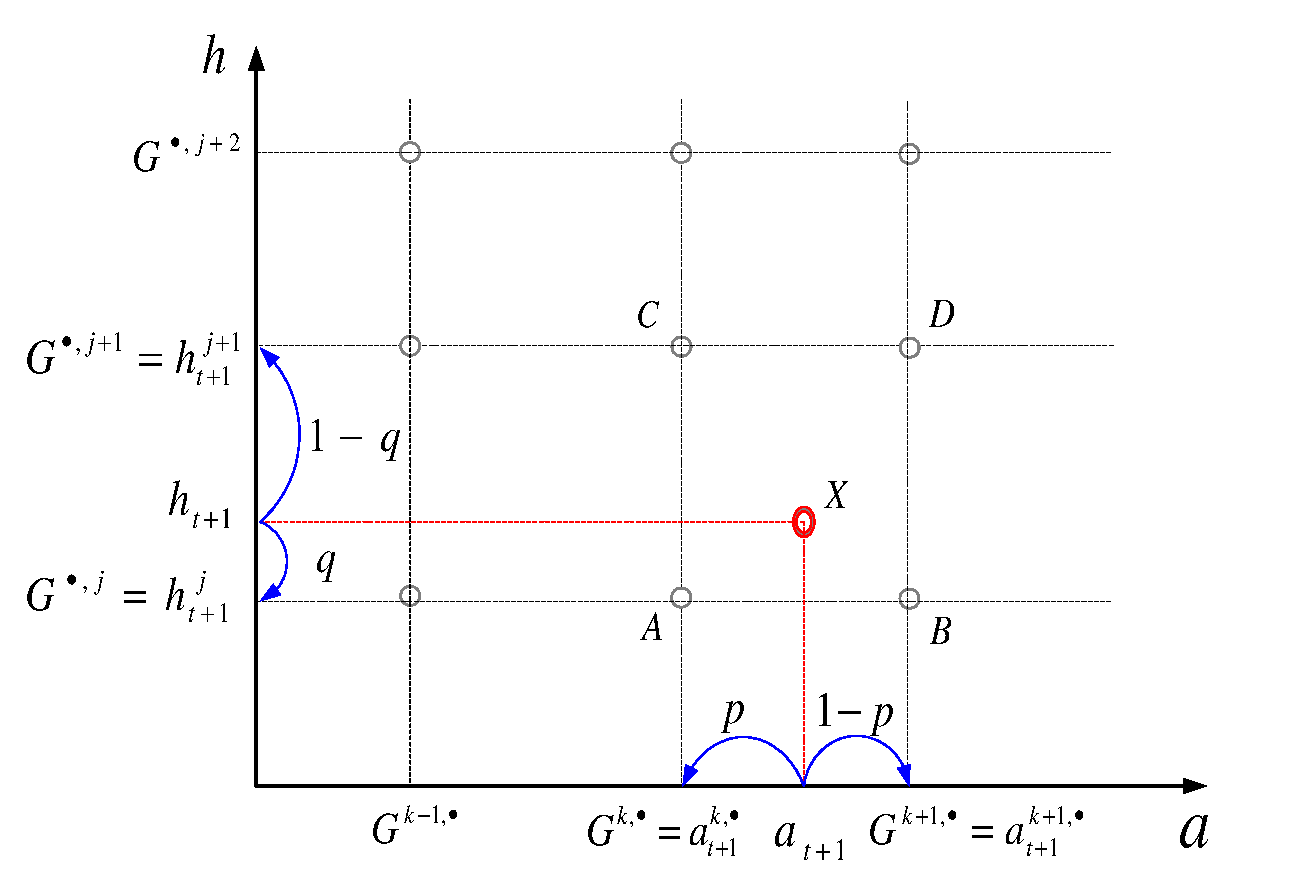
\includegraphics[height=6.0cm, width=9.0cm]{Abbildungen/exo.eps}}}\\
{\footnotesize {Interpolation on rectilinear grids. In any row locate the two columns ($G^{k,\bullet}$ and $G^{k+1,\bullet}$) that form the most narrow bracket of $a_{t+1}$. In any column locate the two rows ($G^{\bullet,j}$ and $G^{\bullet,j+1}$) that form the most narrow bracket of $h_{t+1}$. Interpolation nodes: $(k,j);(k+1,j);(k,j+1);(k+1,j+1)$.}}%
\end{tabular}
\label{Rectilinear_Grid}
\end{figure}

In EXGM, $\mathcal{G}^{a}\otimes\mathcal{G}^{h}$ is predetermined as a rectilinear grid (in every iteration). After locating the nodes bilinear interpolation of any function of~$F$---in our case the value function in~$t$ as well as its first derivatives with respect to~$a$ and~$h$--- at point X requires computing $F\left(  X\right)  =\varphi_{A}F(A)+\varphi_{B}F(B)+\varphi_{C}F(C)+\varphi_{D}F(D)$ with the four basis functions $\varphi$ where
\begin{align*}
\varphi_{A}  &  =p\ast q\\
\varphi_{B}  &  =\left(  1-p\right)  \ast q\\
\varphi_{C}  &  =p\ast\left(  1-q\right) \\
\varphi_{D}  &  =\left(  1-p\right)  \ast\left(  1-q\right)
\end{align*}
with $p=\frac{a_{X}-a_{A}}{a_{B}-a_{A}}$ and $q=\frac{h_{X}-h_{A}}{h_{C}%
-h_{A}}$, cf. \citeN{judd98}.

\subsection{Analytical Solution with Delaunay Interpolation \newline(ENDGM)}

\label{ss:analendgm}

The above setting has a straightforward economic interpretation. Given an exogenous state today $\left(  a_{t},h_{t}\right)$ compute the endogenous control variables $\left( a_{t+1},h_{t+1}\right)  $. The main idea of ENDGM is to redefine exogenous and endogenous objects in the numerical solution: the control variable is taken as exogenous whereas today's state is taken endogenous. In this sense, \textquotedblleft Endogenous Grid Method\textquotedblright\ is a misnomer because computation is still based on an exogenous grid, not for the state but for the control variables.\footnote{A more appropriate name might be \textquotedblleft Endogenous State Grid Method\textquotedblright.}

Computationally we first condition on a set of future endogenous state variables, $\left(  a_{t+1},h_{t+1}\right)$,---which are control variables from the perspective of the current period---and exploit the system of FOCs to determine the corresponding set of contemporaneous controls, $\left( c_{t},i_{t}\right)$. Second, we use the budget constraint and the law of motion for human capital to get the according current set of endogenous state variables, $\left(  a_{t},h_{t}\right)$. Precisely, the implementation steps are as follows:

\begin{enumerate}
\item To initialize ENDGM predefine two grids, one for gross savings $s$, $G^{s}\equiv\left\{  s^{1},s^{2},...,s^{K}\right\}$ which is defined as $s=a_{t}+wh_{t}-c_{t}-i_{t}=\frac{a_{t+1}}{R}$ and one for human capital $z$, $G^{z}\equiv\left\{  z^{1},z^{2},...,z^{J}\right\}$ which is defined as $z=h_{t}+f\left(  i_{t}\right) =\frac{h_{t+1}}{1-\delta}$ and form $\mathcal{G}^{s,z}=\mathcal{G}^{s}\otimes\mathcal{G}^{z}$

\item Define $\mathcal{G}^{a,h}=\mathcal{G}^{a}\otimes\mathcal{G}^{h}$ for $T$. In period $T$, as in EXGM, 
\begin{align*}
c_{T}\left(  \cdot,\cdot\right)   &  =a_{T}^{k,j}+wh_{T}^{k,j}\\
i_{T}\left(  \cdot,\cdot\right)   &  =0
\end{align*}
for all $\left(  a^{k,j},h^{k,j}\right)  \in\mathcal{G}^{a,h}$ and
\begin{align*}
V_{T}\left(  a_{T}^{k,j},h_{T}^{k,j}\right)   &  =\frac{1}{1-\theta}\left[c_{T}^{k,j}\right]  ^{1-\theta}\\
\text{$V_{T_{a}}$}\left(  a_{T}^{k,j},h_{T}^{k,j}\right)   &  =\left[c_{T}^{k,j}\right]  ^{-\theta}\\
\text{$V_{T_{h}}$}\left(  a_{T}^{k,j},h_{T}^{k,j}\right)   &  =\left[  w+\left(  i_{T}^{k,j}\right)  ^{\alpha}\right]  \left[  c_{T}^{k,j}\right]^{-\theta}=w\left[  c_{T}^{k,j}\right]  ^{-\theta}\text{.}
\end{align*}

\item Iterate backwards from~$t=T-1,...,0$. For each $\left(  s^{k},z^{j}\right)  \in\mathcal{G}^{s,z}$:

\begin{enumerate}
\item Compute $a_{t+1}^{k}$ and $h_{t+1}^{j}$%
\begin{align*}
a_{t+1}^{k}  &  =Rs^{k},\\
h_{t+1}^{j}  &  =\left(  1-\delta\right)  z^{j}\text{.}%
\end{align*}

\item Given $V_{t+1}$, $V_{t+1_{a}}$ and $V_{t+1_{h}}$ from the previous iteration step, interpolate the value function and its derivatives at $\left(a_{t+1}^{k},h_{t+1}^{j}\right)  $ to get $V_{t+1}\left(  a_{t+1}^{k},h_{t+1}^{j}\right)  $,\newline$V_{t+1_{a}}\left(  a_{t+1}^{k},h_{t+1}^{j}\right)  $ and $V_{t+1_{h}}\left(  a_{t+1}^{k},h_{t+1}^{j}\right)$ using Delaunay interpolation (see below).

\item \label{Advantage ENDGM} Compute $c_{t}^{k,j}$ and $i_{t}^{k,j}$
\begin{align*}
c_{t}^{k,j}  &  =\left[  \beta R\left(  1-\phi\frac{1}{1+\left(1-\delta\right)  z^{j}}\right) \text{$V_{t+1_{a}}$}\left[ \overset{a_{t+1}^{k}}{\overbrace{Rs^{k}}},\overset{h_{t+1}^{j}}{\overbrace{\left(1-\delta\right)  z^{j}}}\right]  \right]  ^{-\frac{1}{\theta}},\\
i_{t}^{k,j}  &  =\left[  \frac{R}{\left(  1-\delta\right)  }\frac{V_{t+1_{a}}\left[  a_{t+1}^{k},h_{t+1}^{j}\right]  }{\frac{\phi}{\left(  1+h_{t+1}^{j}-\phi\right)  \left(  1+h_{t+1}^{j}\right)  }V_{t+1}\left[  a_{t+1}^{k},h_{t+1}^{j}\right]  +V_{t+1_{h}}\left[  a_{t+1}^{k},h_{t+1}^{j}\right]}\right]  ^{-\frac{1}{\alpha}}\text{.}%
\end{align*}


\item Compute $a_{t}^{k,j}$ and $h_{t}^{k,j}$
\begin{align*}
h_{t}^{k,j}  &  =z^{j}-\frac{1}{1-\alpha} \left(  i_{t}^{k,j}\right)^{1-\alpha}\\
a_{t}^{k,j}  &  =s^{k}-wh_{t}^{k,j}+c_{t}^{k,j}+i_{t}^{k,j}\text{.}
\end{align*}

\item Save/Update both the value function and its derivatives%
\begin{align*}
V_{t}\left[  a_{t}^{k,j},h_{t}^{k,j}\right]   &  =\frac{1}{1-\theta}\left[c_{t}^{k,j}\right]  ^{1-\theta}+\beta\left(  1-\phi\frac{1}{1+h_{t+1}^{j}}\right)  V_{t+1}\left[  a_{t+1}^{k},h_{t+1}^{j}\right] \\
V_{t_{a}}\left[  a_{t}^{k,j},h_{t}^{k,j}\right]   &  =\left[  c_{t}^{k,j}\right]  ^{-\theta}\\
V_{t_{h}}\left[  a_{t}^{k,j},h_{t}^{k,j}\right]   &  =\left[  w+ \left(i_{T}^{k,j}\right)  ^{\alpha}\right]  \left[  c_{t}^{k,j}\right]  ^{-\theta}\text{.}
\end{align*}

\end{enumerate}
\end{enumerate}

The clear advantage of ENDGM compared to EXGM becomes obvious in step \ref{Advantage ENDGM}. Because of the redefinition of~$a_{t+1}$ and~$h_{t+1}$ the system of FOCs can be solved for~$c_{t}$ and~$i_{t}$ analytically and hence no numerical root-finder is needed. Furthermore, ENDGM provides, by definition, an exact determination of the range of the borrowing constraint and produces higher accuracy of the solution than EXGM in this region. However, in contrast to the standard one-dimensional problem, the policy function itself in the range where the borrowing constraint is binding does not have a closed form solution in ENDGM.\footnote{In a standard consumption-savings model with only one endogenous continuous state variable the policy function is computed by linearly interpolating between the policy at zero saving and the origin, cf. \citeN{carroll06}.}
In a multi-dimensional setting, the consumption and human capital investment policy functions are not necessarily linear functions of current cash on hand. To accommodate this we set exogenous grid-points in the region of the borrowing constraint and use a one-dimensional root-finder in order to compute the policy function. For more details see the appendix.

\begin{remark}
\label{rem:failureendgm} In contrast to EXGM, ENDGM is not a general method. Suppose we were to adopt a general Ben-Porath human capital function, cf. \citeN{Benporath67}, in which the level of human capital directly affects the productivity of human capital investments, i.e. we replace~$f(i)$ in equation~(\ref{eq:hkaccum}) with~$f(h,i)$. ENDGM is no longer applicable in such a formulation.
\end{remark}

\paragraph{Delaunay Interpolation}

In EXGM the grid is rectilinear by construction whereas in ENDGM the endogenously computed grid~$\mathcal{G}^{a,h}$ is not. This constitutes the main drawback of ENDGM because location of interpolation nodes is not obvious. As illustrated in Figure~\ref{Irregular_Grid}, separating the multi-dimensional problem into several one-dimensional problems is not possible. In each row not just the value of~$a$ changes but also the value of~$h$ so that the concept of bilinear interpolation in a square grid is not applicable. ENDGM hence generates a situation where neighboring points in the state space do not need to be neighboring elements in the grid matrix. 
\begin{figure}[htb] \centering
\caption{Irregular Grid}
\begin{tabular}
[c]{cc}
& \\
Panel (a) & Panel (b)\\
{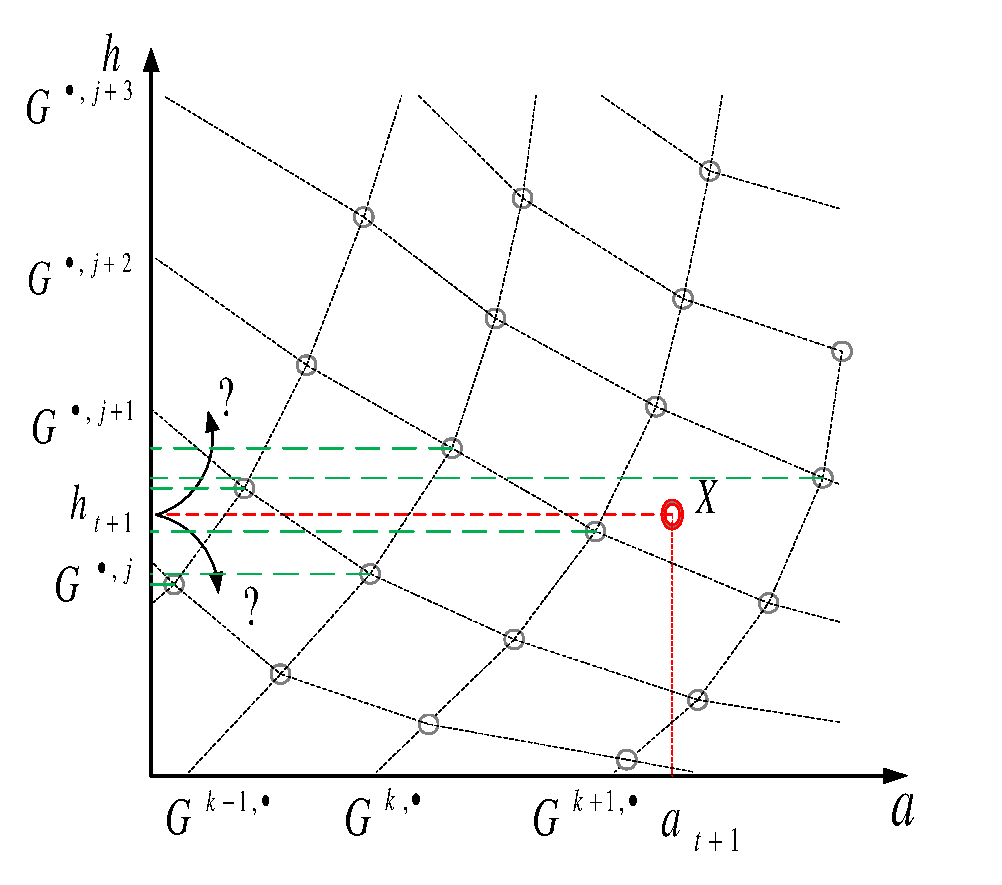
\includegraphics[height=6.0cm, width=7.5cm]{Abbildungen/endo_grid_1.eps}} &
{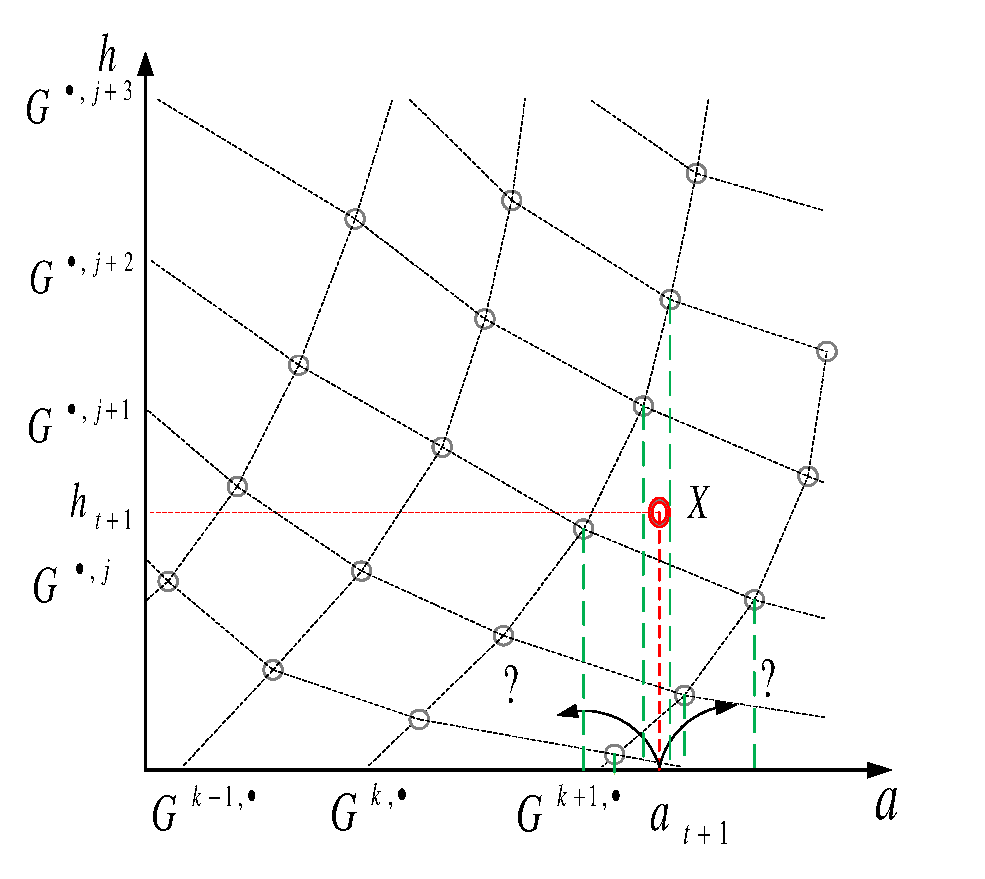
\includegraphics[height=6.0cm, width=7.5cm]{Abbildungen/endo_grid_2.eps}} \\
\multicolumn{2}{p{15cm}}{{\footnotesize Interpolation on irregular grids. Multidimensional interpolation cannot be separated into several one-dimensional interpolations as the values of $a$ and $h$ change in each column or row.}}
\end{tabular}
\label{Irregular_Grid}
\end{figure}

The most common approach adopted in other scientific fields such as geometry or geography to locate neighboring points in an irregular grid is the concept of Delaunay triangulation and its related geometric construct, the Voronoi diagram.\footnote{Recently, these methods have been introduced to Economics, cf., e.g., \citeN{brumm10}}
We explain the geometric construction of the Voronoi diagram by use of figure~\ref{Delaunay Triangulation}. The Voronoi diagram (polygon)---shown in Panel~(a) of Figure~\ref{Delaunay Triangulation}---is the region of the state space consisting of all points closer to gridpoint $P_{1}$ than to any other gridpoint. The Voronoi diagram is obtained from the perpendicular bisectors of the lines connecting neighboring points. Voronoi diagrams for all points form a tessellation of the space, cf. Panel~(a). Edges of the Voronoi diagram are all the points in the plane that are equidistant to the two nearest grid-points, cf. Panel~(b). The Voronoi vertices are the points equidistant to three grid-points, i.e., they are the center of circumcircles including the three neighboring grid-points, cf. Panel~(c). Connecting these grid-points constitutes the unique triangulation known as the Delaunay triangulation as displayed in Panel~(d), cf.\citeN{Baker99}. The vertices of a triangle are the nearest neighbors of all points contained in that triangle. These concepts can also be generalized to more than two dimensions.

\begin{figure}[htb] \centering
\caption{The Voronoi Diagram}
\begin{tabular}
[c]{cc}
& \\
Panel (a) & Panel (b)\\
{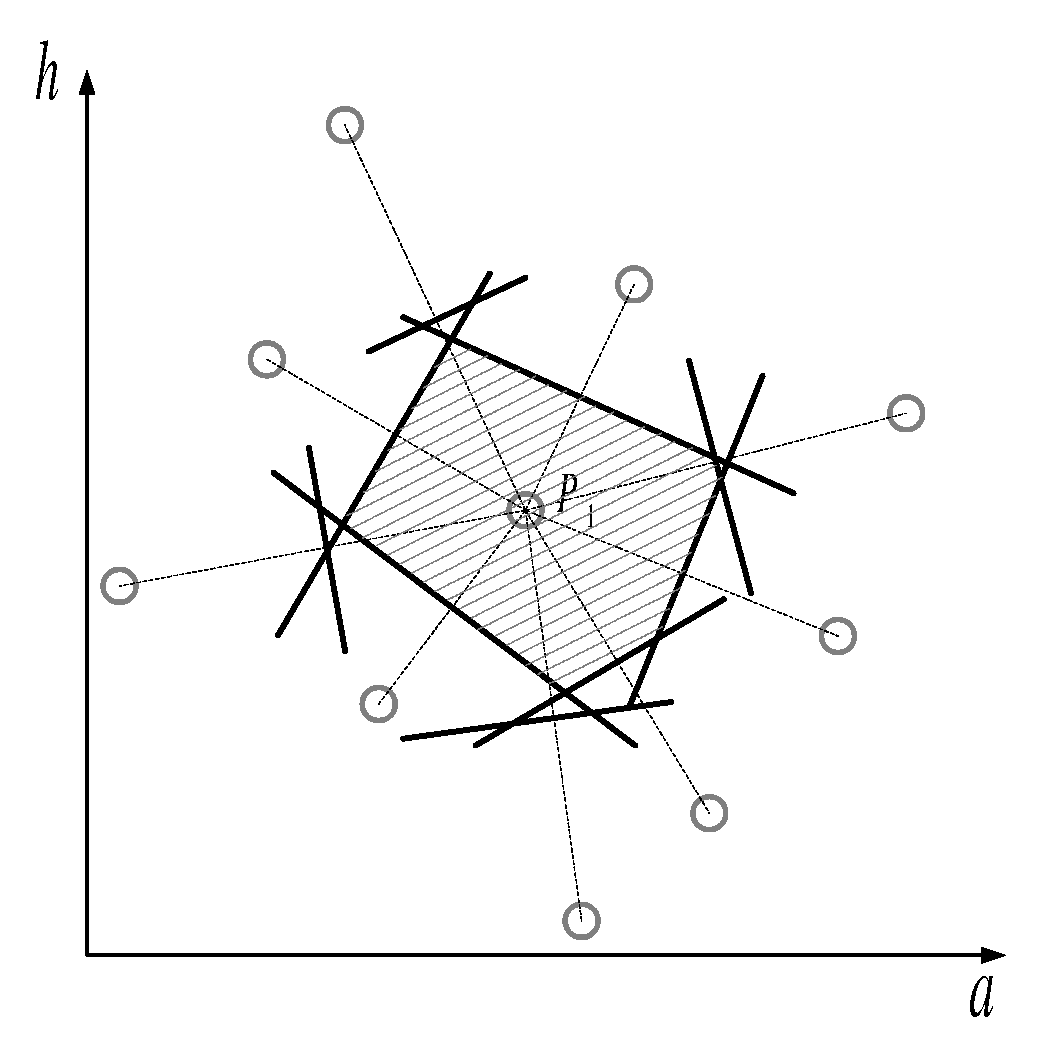
\includegraphics[height=6.0cm, width=6.0cm]{Abbildungen/Voronoi_1_shape.eps}} &
{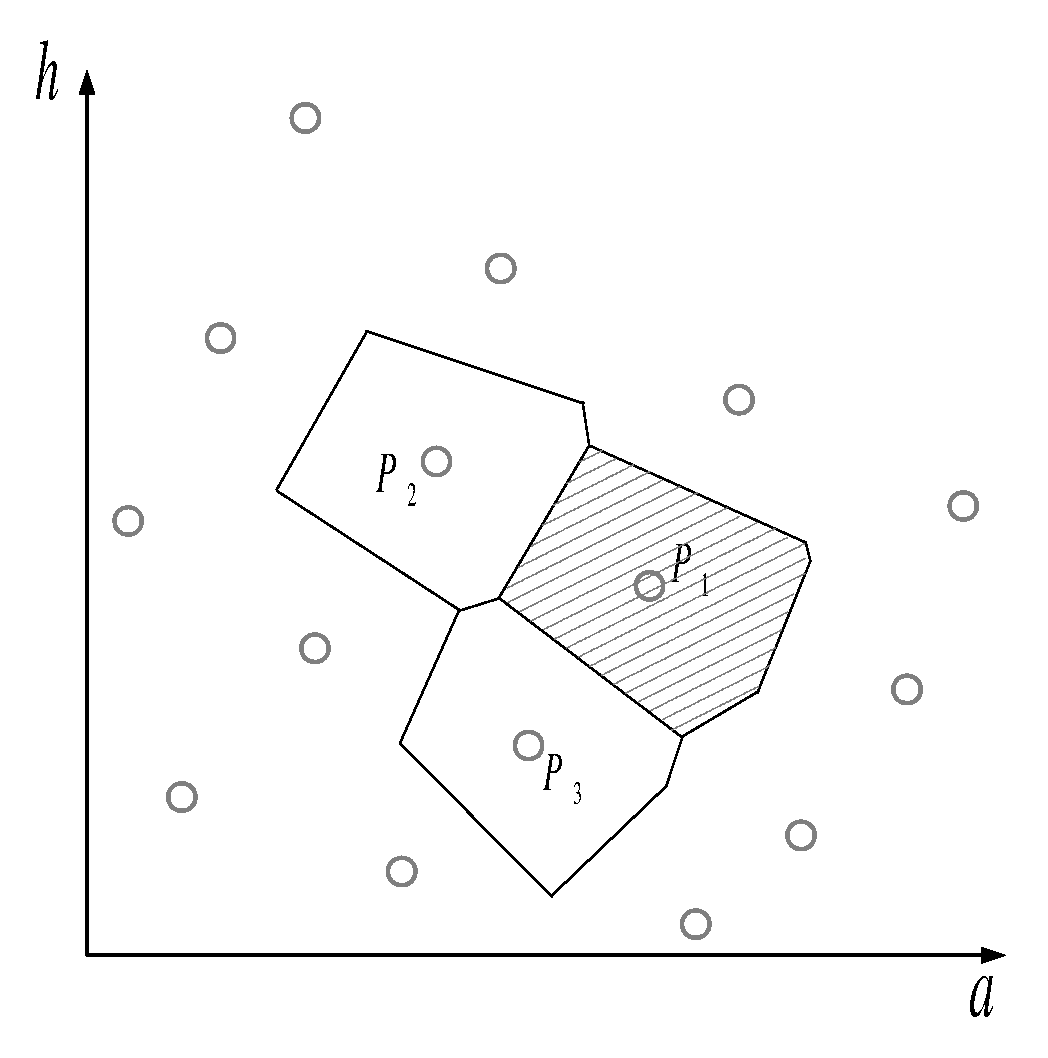
\includegraphics[height=6.0cm, width=6.0cm]{Abbildungen/Voronoi_2_shape.eps}} \\
Panel (c) & Panel (d)\\
{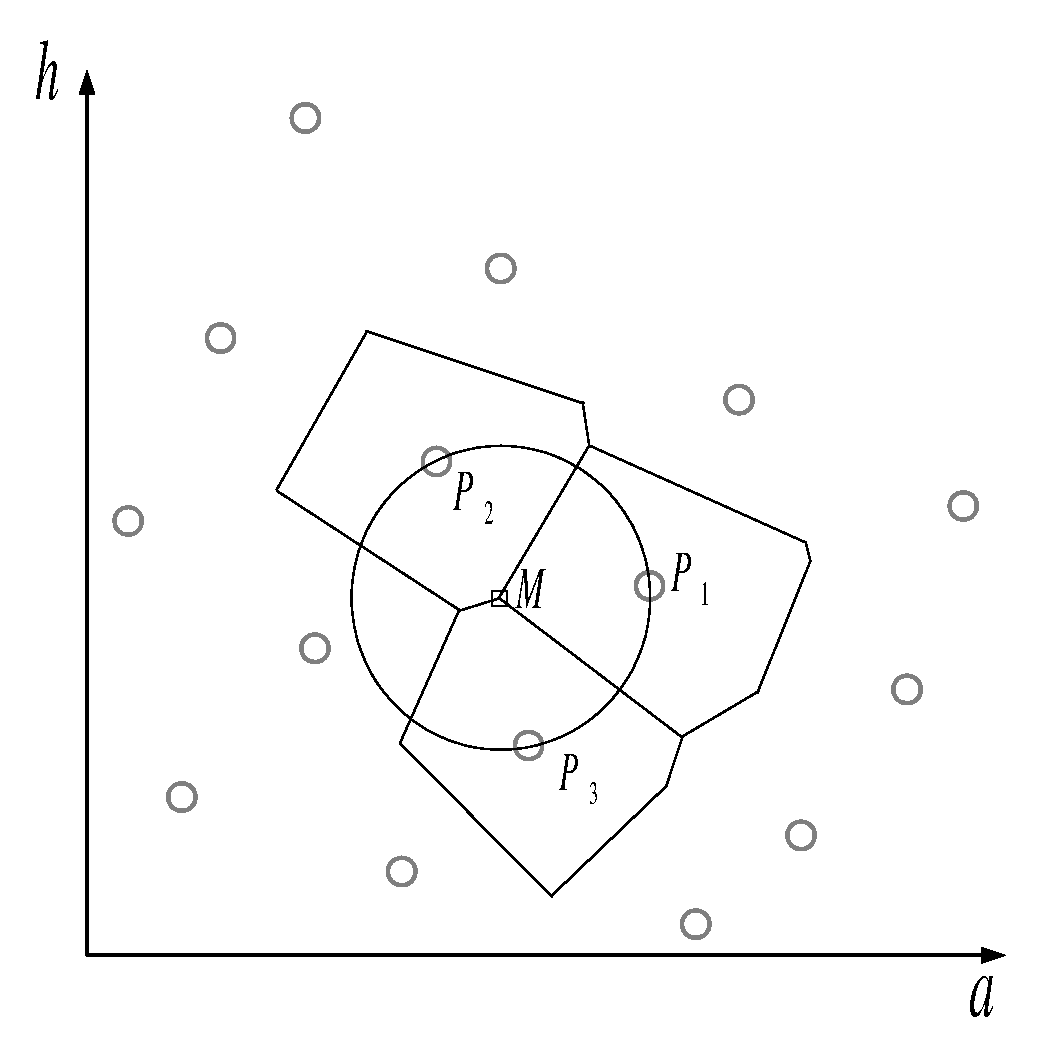
\includegraphics[height=6.0cm, width=6.0cm]{Abbildungen/Voronoi_3.eps}} &
{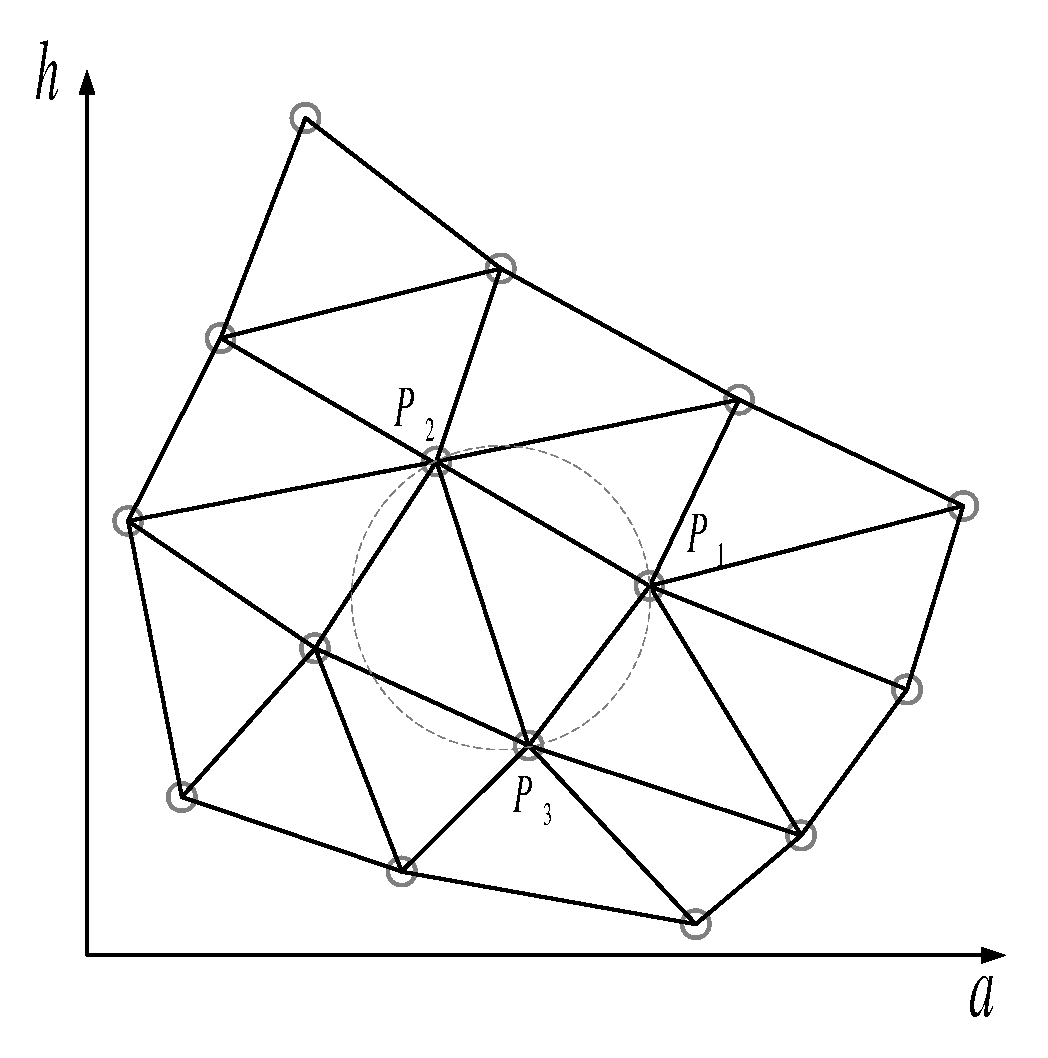
\includegraphics[height=6.0cm, width=6.0cm]{Abbildungen/Delaunay_!.eps}} \\
\multicolumn{2}{p{15cm}}{{\footnotesize Panel (a): Generating the Voronoi polygon: Edges are perpendicular bisectors of lines connecting neighboring points. Panel (b): Several Voronoi tiles in mesh grid. Panel (c): Circle with center at vertex includes three closest points. Panel (d): Delaunay Triangulation: Vertices are nearest neighbors of all points within triangle.}}
\end{tabular}
\label{Delaunay Triangulation}
\end{figure}

The computational implementation of a Delaunay triangulation is done by the so-called randomized incremental algorithm, which we illustrate in Figure~\ref{Delaunay Triangulation Computational}. It is incremental in the sense that it adds points to the triangulation one at a time to maintain a Delaunay triangulation at each stage. It is randomized in that points are added in a random order which guarantees $O(N~log~N)$ expected time for the algorithm, cf.~\shortciteN{numerical3rd}. To construct the Delaunay triangulation for a given point set we initially have to add three ``fictitious'' points $\left[  \Theta_{1},\Theta_{2},\Theta_{3}\right]  $ forming a large starting triangle which encloses all ``real'' points, cf. Panel (a) of Figure~\ref{Delaunay Triangulation Computational}. This is necessary in order to ensure that added points lie within an existing triangle. These ``fictitious'' points are deleted once the triangulation is complete. In each following step of Delaunay triangulation a point from the point set is added to the existing triangulation and connected to the vertices of the enclosing triangle. We illustrate this step in Panel~(b) of the figure. Consider the existing triangle~$P_{1},P_{2},P_{3}$ and a new point from the point set,~$P_{5}$, which is not yet connected to other points. Connecting~$P_{5}$ to~$P_{1}$, $P_{2}$ and $P_{3}$, respectively, gives rise to three new triangles. Next, it is checked whether the newly created triangles are ``legal'', i.e., whether the circumcircle of any triangle does not contain any other point of the point set.\footnote{This principle is derived from the definition that a triangulation fulfills the Delaunay property if and only if the circumcircle of any triangle does not contain a point in its interior, cf.\shortciteN{berg08}.}
In our example, we first visit triangle~$P_{2},P_{3},P_{5}$ in Panel~(c). As shown in the figure, the circumcircle contains point~$P_{4}$. Hence, triangle~$P_{2},P_{3},P_{5}$ is not legal. Therefore, flip the edge opposite of $P_{5}$ connecting~$P_{5}$ with~$P_{4}$. This operation creates two new triangles, $P_{3},P_{4},P_{5}$ and~$P_{2},P_{4},P_{5}$, cf.~Panel~(d) of the figure, which must be checked for legality. In our example, triangle~$P_{3},P_{4},P_{5}$ is legal because the circumcircle does not contain other existing points from the point set. The process is recursive and never wanders away from any point~$P$ (point~$P_{5}$ in our example). The only edges that can be made illegal by inserting a point $P$ are edges opposite $P$ (in triangles with~$P$ as a vertex).\footnote{This procedure is described in \shortciteN{numerical3rd}. We use the numerical package geompack3 based on~\citeN{Joe91} for both the Delaunay triangulation and the ``visibility walk'', described next.}

\begin{figure}[htb] \centering
\caption{Incremental Algorithm}
\begin{tabular}
[c]{cc}
& \\
Panel (a) & Panel (b) \\
{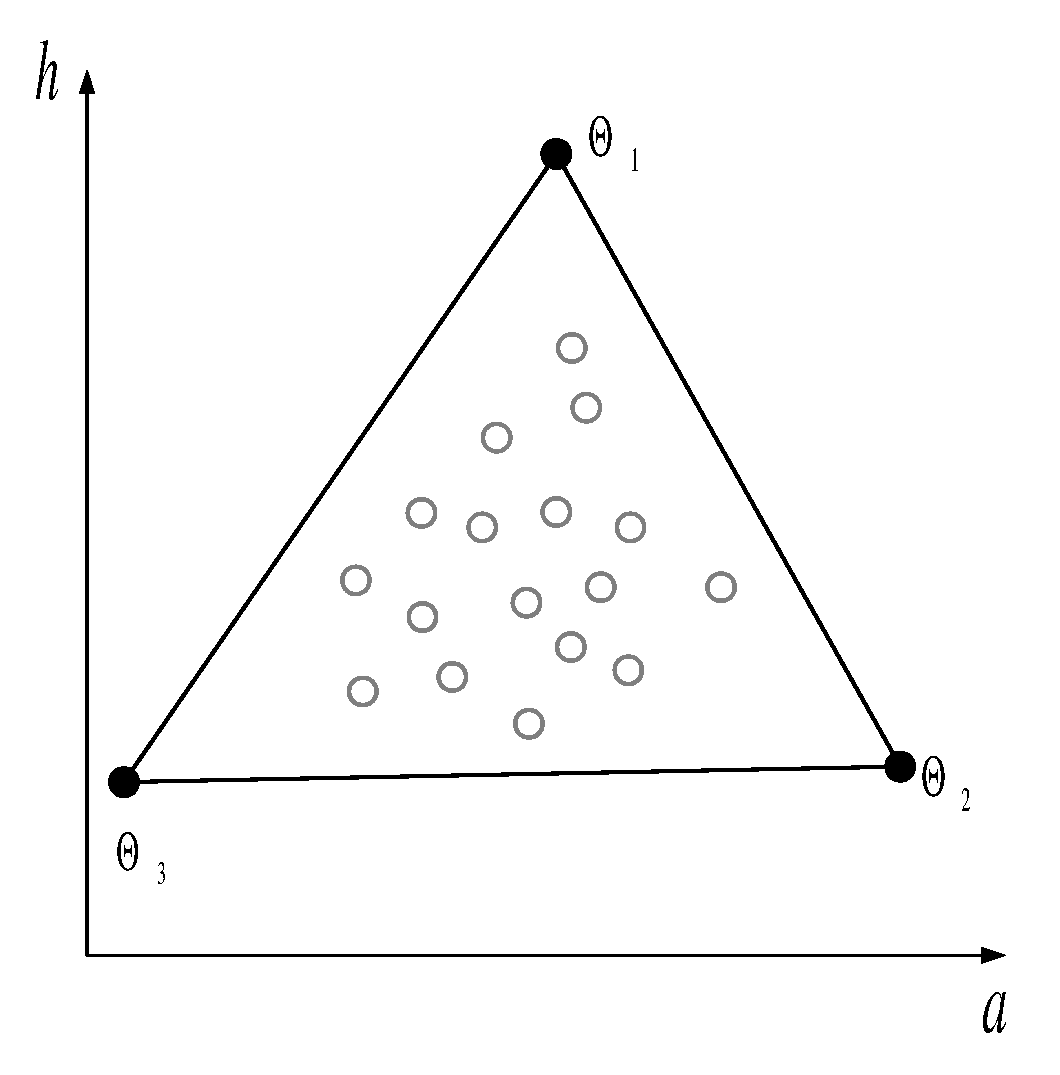
\includegraphics[height=6.0cm, width=6.0cm]{Abbildungen/Incremental_0.eps}} &
{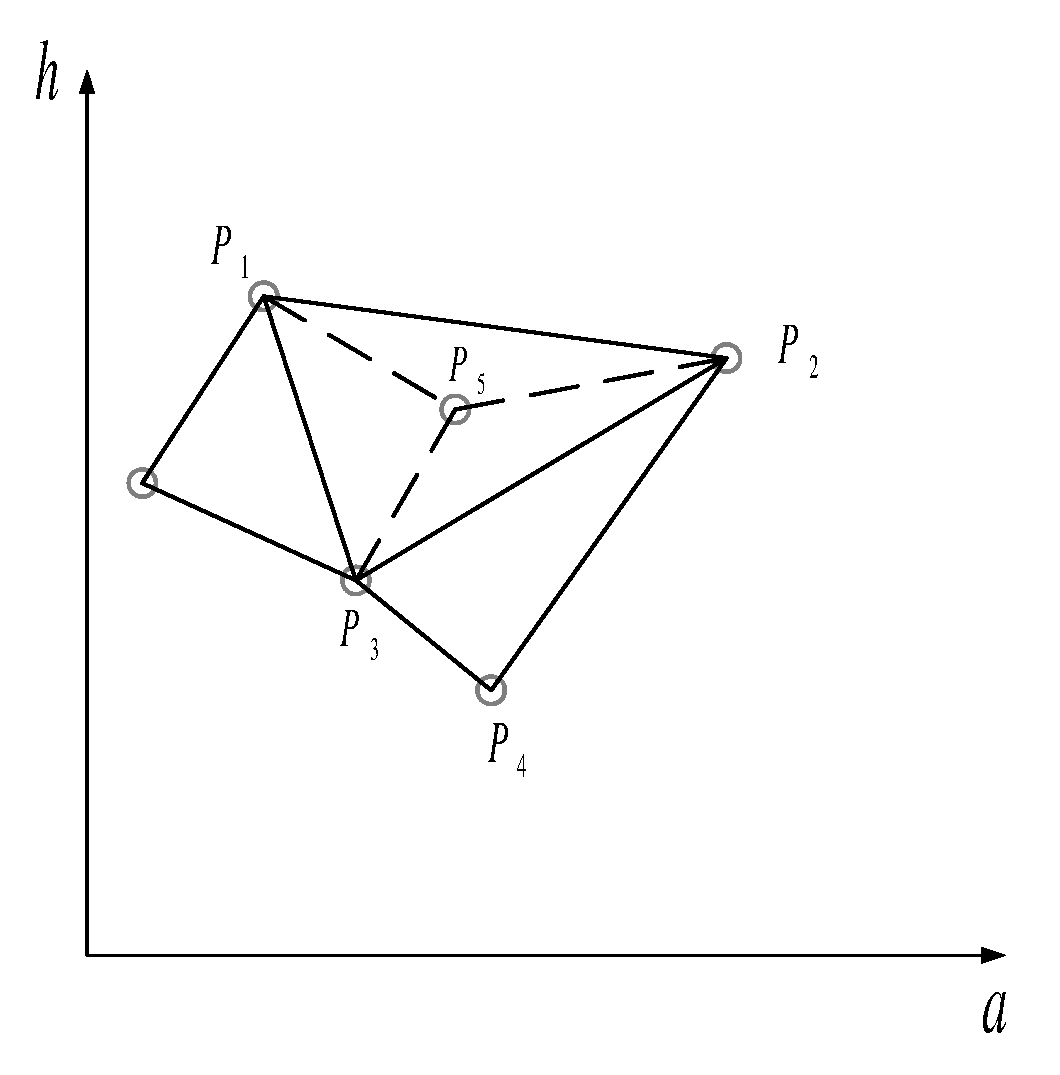
\includegraphics[height=6.0cm, width=6.0cm]{Abbildungen/Incremental_1.eps}} \\
Panel (c) & Panel (d) \\
{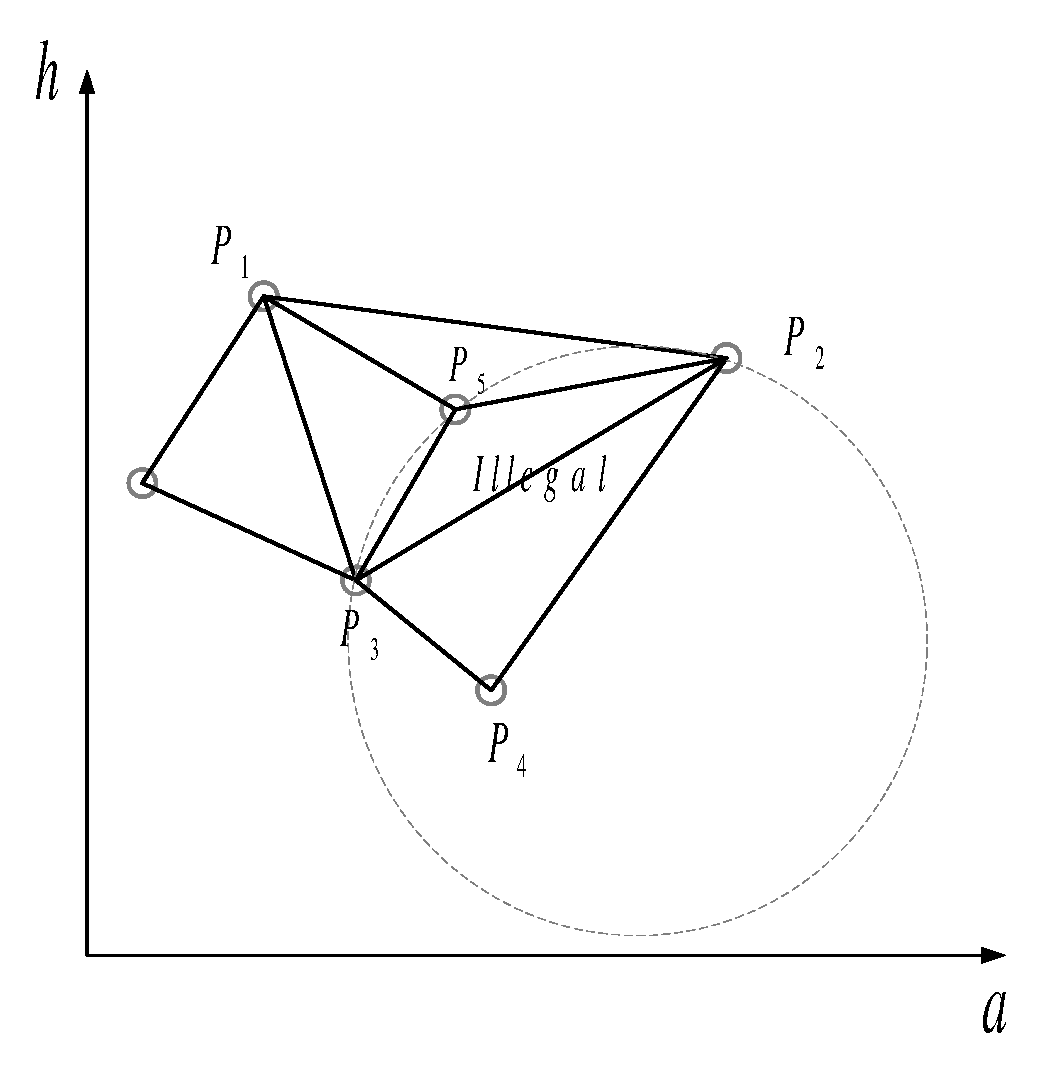
\includegraphics[height=6.0cm, width=6.0cm]{Abbildungen/Incremental_2.eps}} &
{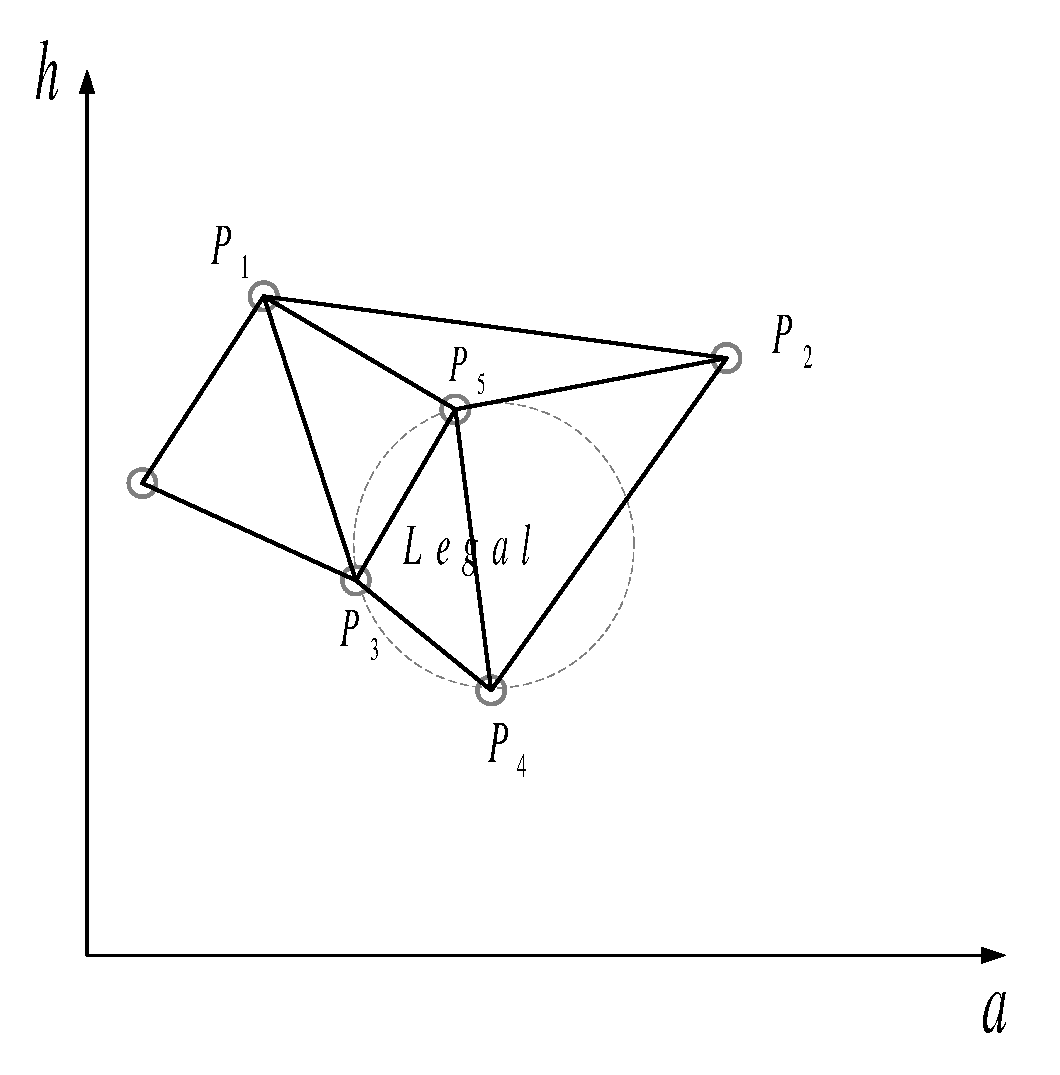
\includegraphics[height=6.0cm, width=6.0cm]{Abbildungen/Incremental_3.eps}} \\
\multicolumn{2}{p{15cm}}{{\footnotesize Panel (a): Three "fictional" points added to constitute the first triangle which includes all "real" points of the point set. Panel (b): Point added to existing Delaunay Triangulation and connected to vertices of enclosing triangle. Panel (c): Circumcircle contains a point. and is therefore illegal triangle. Panel (d): Circumcircle does not contain any point and is therefore legal.}}
\end{tabular}
\label{Delaunay Triangulation Computational}
\end{figure}

At interpolation, to locate a (query) point~$X$ in a given planar triangular mesh we adopt a procedure referred to as visibility walk which is illustrated in Figure~\ref{Visibility walk}. The search starts from an initial guess of a triangle,~$\Delta_{1}$. Then, it is tested if the line supporting the first edge~$e$ separates~$\Delta_{1}$ from the query point~$X$ which reduces to a single operation test. If this is the case, the next triangle being visited is the neighbor of~$\Delta_{1}$ through~$e$, $\Delta_{2}$. Otherwise the second edge is tested in the same way. In case the test for the second edge also fails then the third edge is tested. The failure of this third test means that the goal has been reached. In Figure~\ref{Visibility walk}, this would be the case at triangle $\Delta_{X}$ which contains $X$.\footnote{In non-Delaunay triangulations, the visibility walk may fall into a cycle, whereas in Delaunay triangulations the visibility walk always terminates, cf.~\shortciteN{Devillers01}.}
\shortciteN{Devillers01} find that performance of the visibility walk is better than other possible algorithms. The location step for the visibility walk takes only $O\log\left(N\right)$ operations, cf.~\shortciteN{numerical3rd}. The starting triangle may be arbitrary. However, an informed choice may radically shorten the length of the walk. We accommodate this by initializing the search with our solutions to grid-points visited previously.

\begin{figure}[htb] \centering
\caption{Visibility Walk}
\begin{tabular}
[c]{p{15cm}}
\\
\multicolumn{1}{c}{{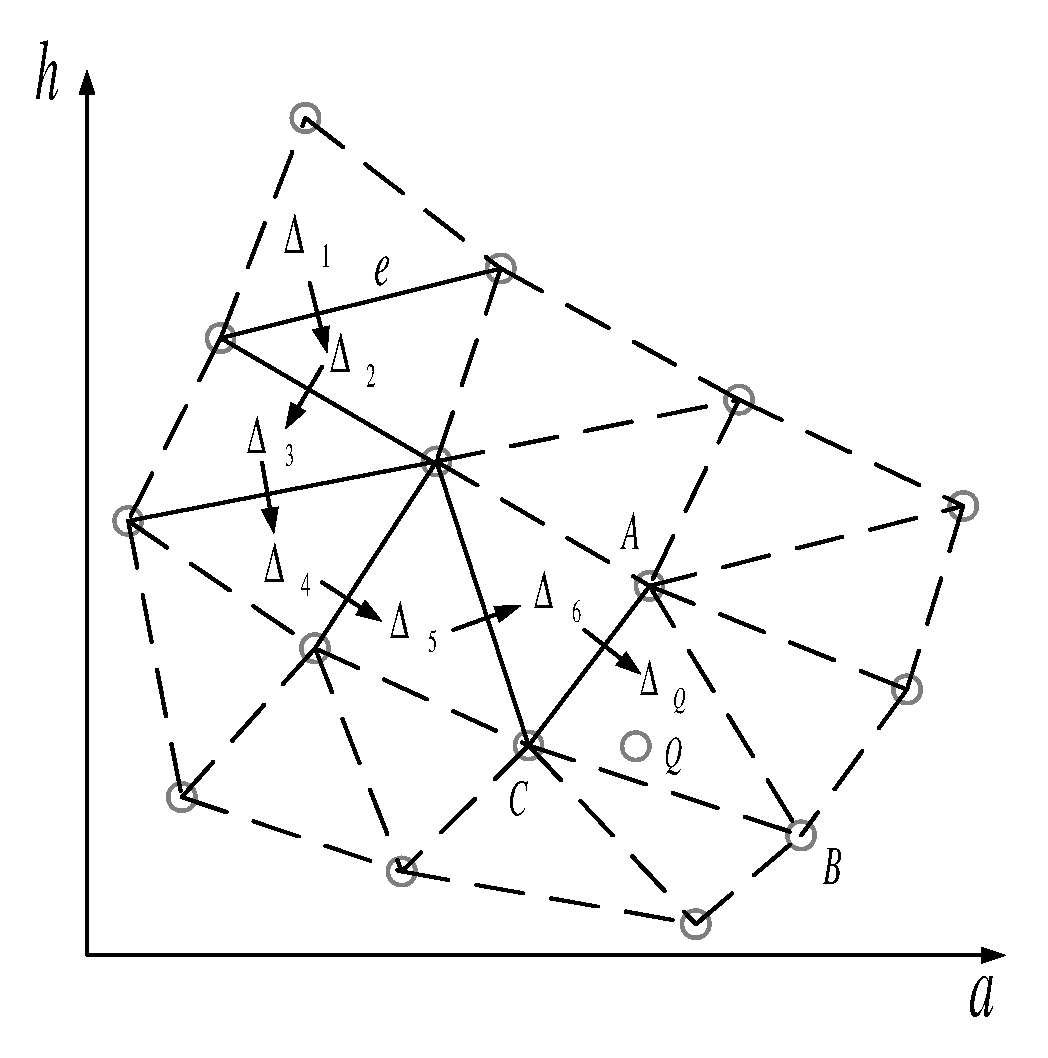
\includegraphics[height=6.0cm, width=7.5cm]{Abbildungen/visibility_walk_2.eps}}} \\
{\footnotesize Visibility walk in Delaunay triangulation - Locate triangle $\Delta_{X}$ containing $X$ with initial guess $\Delta_{1}$. If the line supporting $e$ separates $\Delta$ from $X$, which reduces to a single orientation test, then the next visited triangle is the neighbor of $\Delta$ through $e$.}
\end{tabular}
\label{Visibility walk}
\end{figure}

After locating the triangle we compute the normalized barycentric coordinates (weights) of the query point $X$ with respect to the vertices $(A,B,C)$ of the triangle $\Delta_{X}$
\begin{align*}
\varphi_{A}  &  =\frac{\left(  a_{X}-a_{C}\right)  \left(  h_{B}-h_{C}\right)+\left(  a_{C}-a_{B}\right)  \left(  h_{X}-h_{C}\right)  }{\left(  a_{A}-a_{C}\right)  \left(  h_{B}-h_{C}\right)  +\left(  a_{C}-a_{B}\right)\left(  h_{A}-h_{C}\right)  }\\
\varphi_{B}  &  =\frac{\left(  a_{X}-a_{C}\right)  \left(  h_{C}-h_{A}\right)+\left(  a_{A}-a_{C}\right)  \left(  h_{X}-h_{C}\right)  }{\left(  a_{A}-a_{C}\right)  \left(  h_{B}-h_{C}\right)  +\left(  a_{C}-a_{B}\right)\left(  h_{A}-h_{C}\right)  }\\
\varphi_{C}  &  =1-\varphi_{A}-\varphi_{B}.
\end{align*}
Finally, the interpolated value of any function~$F$ at point $X$ is given as the weighted average of the respective function values at the vertices,
\[
F\left(  X\right)  =\varphi_{A}F(A)+\varphi_{B}F(B)+\varphi_{C}F(C).
\]

\subsection{One-Dimensional Root-Finding with Hybrid Interpolation (HEGM)}

We next consider a hybrid method (HEGM) which combines EXGM and ENDGM. Specifically, we use ENDGM in one dimension of the problem only. Hence, we define one of the two state variables on an \textquotedblleft endogenous\textquotedblright\ grid, whereas the other is on an \textquotedblleft exogenous\textquotedblright\ grid. The algorithm proceeds in three steps. In the first step, conditioning on control variable~$a_{t+1}$ and current state~$h_{t}$, we exploit one of the two FOCs to derive one policy function---in this setup investment in human capital,~$i_{t}$. In this step a one-dimensional solver is required. To preserve comparability with the previously described methods we choose Broyden's method.\footnote{Using Brent's method instead turns out to slow down speed of HEGM.}
In the second step, policy function~$i_{t}$ is used to get the second endogenous state variable,~$h_{t+1}$. Exploiting the second FOC we get the second policy function,~$c_{t}$. In the third step, we compute the corresponding state variable~$a_{t}$ from the budget constraint. The implementation steps are as follows:

\begin{enumerate}
\item To initialize HEGM predefine two grids, one for gross savings $s$, $\mathcal{G}^{s}\equiv\left\{  s^{1},s^{2},...,s^{K}\right\}  $ and one for human capital $h$, $\mathcal{G}^{h}\equiv\left\{ h^{1},h^{2},...,h^{J}\right\}$ and form $\mathcal{G}^{s,h}=\mathcal{G}^{s}\otimes\mathcal{G}^{h}$

\item In period~$T$, define an initial guess for $\mathcal{G}^{a,h}=\mathcal{G}^{a}\otimes\mathcal{G}^{h}$ and compute
\begin{align*}
c_{T}\left( \cdot,\cdot\right)  &  =a_{T}^{k,j}+wh_{T}^{j}\\
i_{T}\left( \cdot,\cdot\right)  &  =0
\end{align*}
for all $\left(  a_{T}^{k,j},h_{T}^{j}\right)  \in\mathcal{G}^{a,h}$ and
\begin{align*}
V_{T}\left(  a_{T}^{k,j},h_{T}^{j}\right)  &  =\frac{1}{1-\theta}\left[c_{T}^{k,j}\right]  ^{1-\theta}\\
\text{$V_{T_{a}}$}\left( a_{T}^{k,j},h_{T}^{j}\right)  &  =\left[ c_{T}^{k,j}\right]^{-\theta}\\
\text{$V_{T_{h}}$}\left( a_{T}^{k,j},h_{T}^{j}\right)  &  =\left[ w+\left(i_{T}^{k,j}\right)^{\alpha}\right] \left[  c_{T}^{k,j}\right]^{-\theta}.
\end{align*}

\item Given functions $V_{t+1}$, $V_{t+1_{a}}$ and $V_{t+1_{a}}$ from the previous step iterate backwards on $t=T-1,...,0$. For each\ $\left(s^{k},h^{j}\right)  \in\mathcal{G}^{s,h}$:

\begin{enumerate}
\item \label{HEGM solver}Solve the one-dimensional equation system for $i_{t}^{k,j}$
\[
i_{t}^{k,j}=\left[  \frac{R}{\left(  1-\delta\right)  }\frac{\text{$V_{t+1_{a}} $}\left[  \overset{a_{t+1}^{k}}{\overbrace{Rs^{k}}},\overset{h_{t+1}^{k,j}}{\overbrace{\left( 1-\delta\right)  \left(h_{t}^{j}+\frac{1}{1-\alpha}\left( i_{t}^{k,j}\right)  ^{1-\alpha}\right)}}\right]  }{\frac{\phi}{\left( 1+h_{t+1}^{k,j}-\phi\right)  \left( 1+h_{t+1}^{k,j}\right)}V_{t+1}\left[ a_{t+1}^{k},h_{t+1}^{k,j}\right] +\text{$V_{t+1_{h}}$}\left[a_{t+1}^{k},h_{t+1}^{k,j}\right] }\right]^{-\frac{1}{\alpha}}
\]
using Broyden's method.\ This includes several computations of $a_{t+1}^{k}$ and $h_{t+1}^{k,j}$ and hybrid interpolations---described below---on $V_{t+1}$, $V_{t+1_{a}}$and $V_{t+1_{h}}$.

\item Use $i_{t}^{k,j}$ to compute
\[
h_{t+1}^{k,j}=\left(  1-\delta\right)  \left(  h_{t}^{j}+\frac{1}{1-\alpha}\left(  i_{t}^{k,j}\right)  ^{1-\alpha}\right)
\]
and next compute $c_{t}^{k,j}$ as
\[
c_{t}^{k,j}=\left(  \beta R\left(  1-\phi\frac{1}{1+h_{t+1}^{k,j}}\right)\text{$V_{t+1_{a}}$}\left[  Rs^{k},h_{t+1}^{k,j}\right]  \right)  ^{-\frac{1}{\theta}}.
\]

\item Compute $a_{t}^{k,j}$ from the budget constraint, hence
\[
a_{t}^{k,j}=s^{k}-wh_{t}^{j}+c_{t}^{k,j}+i_{t}^{k,j}.
\]


\item Save/Update both the value function and its derivatives
\begin{align*}
V_{t}\left(  a_{t}^{k,j},h_{t}^{j}\right) &  =\frac{1}{1-\theta}\left[c_{t}^{k,j}\right]  ^{1-\theta}+\beta\left(  1-\phi\frac{1}{1+h_{t+1}^{k,j}}\right)  V_{t+1}(a_{t+1}^{k},h_{t+1}^{k,j})\\
\text{$V_{t_{a}}$}\left(  a_{t}^{k,j},h_{t}^{j}\right)   &  =\left[c_{t}^{k,j}\right]  ^{-\theta}\\
\text{$V_{t_{h}}$}\left(  a_{t}^{k,j},h_{t}^{j}\right)   &  =\left[  w+\left(i_{T}^{k,j}\right)  ^{\alpha}\right]  \left[  c_{t}^{k,j}\right]  ^{-\theta}.
\end{align*}

\end{enumerate}
\end{enumerate}

As EXGM, HEGM requires to run a numerical solver~$\left[  K\ast J\right]$ times. However, computational burden is alleviated by reducing complexity of the equation system. Furthermore, as in ENDGM, it is possible to exactly determine the range of the borrowing constraint. In contrast to ENDGM in two dimensions, there is no need for a complex interpolation method.

\begin{remark}
\label{rem:failurehegm} As ENDGM, HEGM is not a general method. Suppose that consumption has an additional effect on human capital. Correspondingly rewrite~(\ref{eq:hkaccum}) to~$h_{t+1}=\left(  1-\delta\right)$ $\left(h_{t}+f(i_{t})-g\left( c_{t}\right) \right)$ to the effect that both controls~$c_{t}$ and~$i_{t}$ appear on both sides of the equation system even after applying the reformulation of endogenous states. This renders HEGM inapplicable.\footnote{\citeN{Hintermaier10} show a potential way to solve this specific problem by a different kind of HEGM. \citeANP{Hintermaier10} replace the numerical solver in step~\ref{HEGM solver} with an additional outer loop over a guess for a future endogenous state. In finite horizon models, this procedure requires an exact knowledge of the state in the last period. In a durable goods model, \citeANP{Hintermaier10} set both states to zero in the last period T+1. In a human capital model such as ours such an assumption is however invalid. It can only be assumed that optimal investment in human capital is zero in the last period but not the human capital stock itself.}
\end{remark}

\paragraph{Hybrid Interpolation}

Hybrid interpolation, illustrated in Figure~\ref{Hybrid interpolation}, is defined on a curvilinear grid where one dimension is being held constant. To locate any query point $X$ hybrid interpolation proceeds in three steps. First, in the dimension of the exogenous grid (current state~$h_{t}$) find the most narrow bracket of $h_{t+1}$ and compute the weights according to the relative distance to these grid-points. Second, in both rows, find those grid-points that form the most narrow bracket of~$a_{t+1}$ and compute the according weights. Third, interpolation of any function of~$F$ at\ point $X$ requires computing $F\left(  X\right)  =\varphi_{A}F(A)+\varphi_{B}F(B)+\varphi_{C}F(C)+\varphi_{D}F(D)$ with the four basis functions $\varphi$ where
\begin{align*}
\varphi_{A}  &  =p\ast q\\
\varphi_{B}  &  =\left(  1-p\right)  \ast q\\
\varphi_{C}  &  =r\ast\left(  1-q\right) \\
\varphi_{D}  &  =\left(  1-r\right)  \ast\left(  1-q\right)
\end{align*}
with $p=\frac{a_{X}-a_{A}}{a_{B}-a_{A}}$, $r=\frac{a_{X}-a_{C}}{a_{D}-a_{C}}$ and $q=\frac{h_{X}-h_{C}}{h_{C}-h_{A}}$. Thus, HEGM reduces complexity of the problem without involving advanced interpolation procedures.

\begin{figure}[htb] \centering
\caption{Hybrid Interpolation}
\begin{tabular}
[c]{p{15cm}}
\\
\multicolumn{1}{c}{{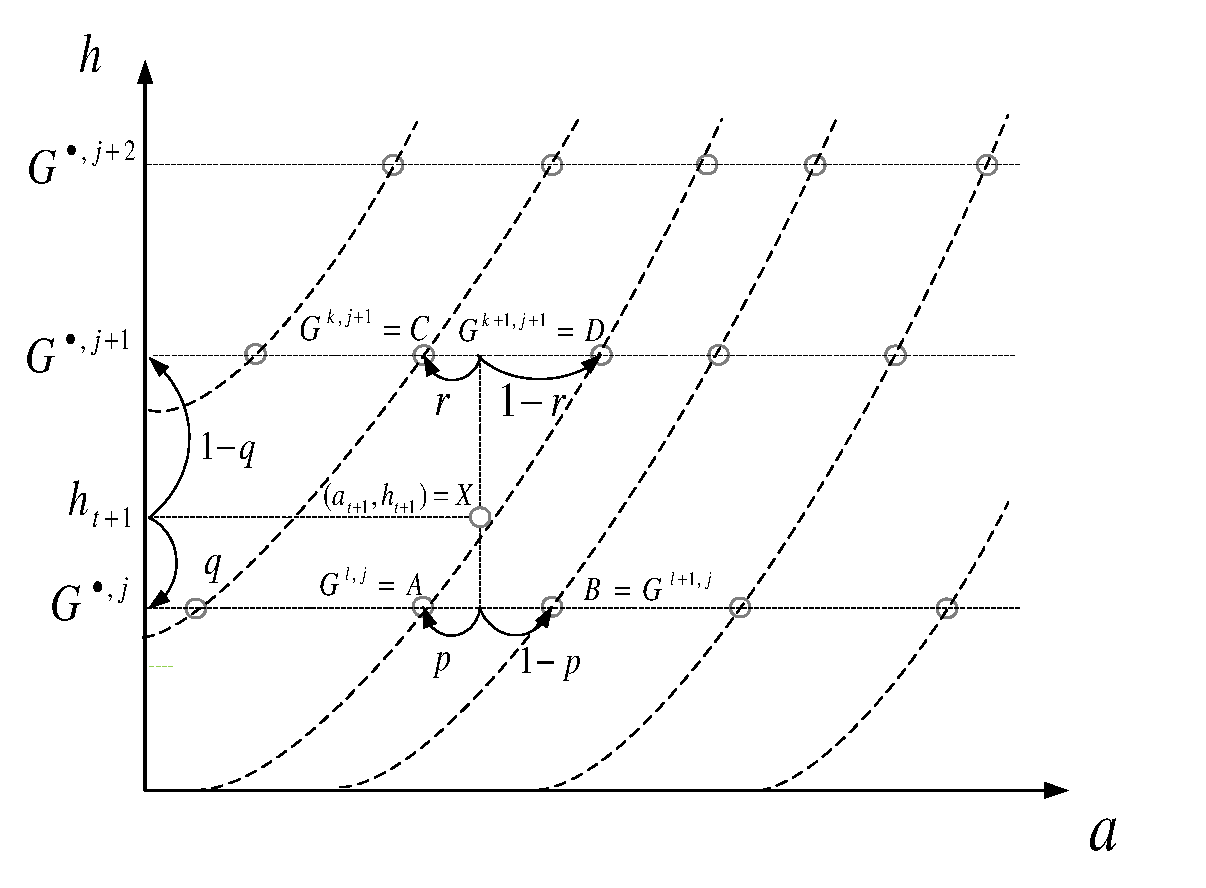
\includegraphics[height=6.0cm, width=9.0cm]{Abbildungen/hybrid_3.eps}}}\\
{\footnotesize Hybrid Interpolation. First, in the exogenous dimension, locate the two rows $G^{\bullet,j}$ and $G^{\bullet,j+1}$ that form the most narrow bracket of $h_{t+1}$. Second, locate in these two rows the grid-points that form the most narrow bracket of $a_{t+1}$. Interpolation nodes: $(k,j)$; $(k,j+1)$; $(l,j+1)$; $(l+1,j+1)$.}
\end{tabular}
\label{Hybrid interpolation}
\end{figure}

\section{Results}

We present results separately for the finite and infinite horizon versions of our model. Throughout, we use triple exponential grids for $a$, $h$, $s$, $z$, respectively. We set the range of grid $G_{s}$ to $\left[ 0,500\right]$ and the range of $G_{z}$ to $\left[ 1,5300\right]$. The according grids $G_{a}$ and $G_{h}$ are adjusted to cover the corresponding range of the state space.

\subsection{Finite Horizon}

We iterate over $T=100$ time periods. Computational speed of the respective algorithms is measured in seconds. Evaluation of accuracy of the solution is done by applying normalized Euler equation errors, cf.~\citeN{judd92}, as has become standard in the literature, cf., e.g.,~\citeN{Santos2000} and~\citeN{Barillas07}. In our approach we get the Euler equation errors $e_{1}$ and $e_{2}$ by
using the respective envelope conditions and combine them with the FOCs to
get:
\begin{align*}
e_{1} & = 1 - \frac{\left[R s(h_{t+1}) \beta \left(c_{t+1}\right)^{-\theta}\right]^{-\frac{1}{\theta}}}{c_{t}}, \\
e_{2} & = 1 - \frac{\left[\frac{R}{\left(1 - \delta\right)} \left(\frac{s_{h}(h_{t+1}) V_{t+1}}{s(h_{t+1})\left(c_{t+1}\right)^{-\theta}} + w + \frac{1}{\left(i_{t+1}\right)^{-\alpha}}\right)^{-1}\right]^{-\frac{1}{\alpha}}}{i_{t}}.
\end{align*}
This error is a dimension free quantity expressing the optimization error as a fraction of current consumption. An error of $e_{1}=10^{-3}$, for instance, means the household would make a \$1 mistake for each \$1000 spent, cf.~\citeN{aruoba06}. These errors are expressed in units of base 10-logarithm which means that $-4$ is an error of $0.0001$. To compare these methods in terms of accuracy we simulate 100 life-cycles profiles. Initial assets $a_{0}$ are set in the range $\{10,100\}$ whereas initial human capital $h_{0}$ differs in the range $\{50,100\}$. For each age we compute $e_{1}$ and $e_{2}$.

Averages and maximum errors are provided in Table~\ref{results_finite}. Both are of similar magnitudes across algorithms. To evaluate the relative performance of the different algorithms, we can therefore further concentrate on comparison speed only.

Table~\ref{results_finite} shows computing times for EXGM, ENDGM and HEGM for different numbers of grid-points. As can further be seen in Panel~(a) of~Figure~\ref{graph_finte} EXGM is outperformed by both ENDGM and HEGM. Furthermore, we experience numerical stability problems with EXGM, especially for large number of grid-points.\footnote{Similar problems are documented by~\citeN{Hintermaier10}.}
Handling the applied numerical routines becomes cumbersome and finding a solution is not guaranteed. If possible, EXGM should therefore be avoided in higher dimensional problems.

Panel~(b) of Figure~\ref{graph_finte} shows that ENDGM has a relative advantage in comparison to HEGM in solving the model with a relatively small number of grid-points. At a grid size of~$20^{2}$, ENDGM is more than~$1.6$ times faster than HEGM. For solving the model with a higher number of grid-points, however, HEGM is advantageous. At a grid size of~$300^{2}$ HEGM is more than 1.3 times faster than ENDGM. In our setting the break-even point between both algorithms is at a number of~$180^{2}$ grid-points and a computing time of~$8.2s.$ As can be seen from Table~\ref{results_finite}, for a standard choice of~$20$ to~$40$ grid-points in each dimension, ENDGM is $\frac{0.421}{0.296}\approx1.4$ to~$\frac{0.125}{0.078}\approx1.6$ times faster than HEGM and $\frac{0.156}{0.078}\approx2$ to~$\frac{0.624}{0.296}\approx2.1$ times faster than EXGM.

\begin{table}[htb] \centering
\caption{Finite Horizon Model: Speed}
\begin{tabular}{L{3.5cm}||C{2cm}|C{2cm}|C{3cm}|C{3cm}}
\multicolumn{5}{p{14cm}}{}\\
& \multicolumn{2}{c|}{Speed} & \multicolumn{2}{c}{Euler error for $\left(c;i\right)$} \\ 
Number of Grid- points for $(a,h)$ & Seconds & Relative to ENDGM & Maximum & Average \\ \hline
ENDGM &  &  &  & \\
$\left(  20,20  \right)$ &  $0.078$ &    -    & $(-2.45;\ -1.98)$ & $(-3.91;\ -2.87)$ \\
$\left(  40,40  \right)$ &  $0.296$ &    -    & $(-2.83;\ -2.41)$ & $(-4.44;\ -3.44)$ \\
$\left( 100,100 \right)$ &  $2.122$ &    -    & $(-3.34;\ -3.16)$ & $(-5.08;\ -4.06)$ \\
$\left( 200,200 \right)$ & $10.546$ &    -    & $(-4.32;\ -3.61)$ & $(-5.60;\ -4.55 )$ \\
&  &  &  & \\ \hline
HEGM &  &  &  &  \\
$\left(  20,20  \right)$ &  $0.125$ & $1.603$ & $(-2.62;\ -2.13)$ & $(-3.92;\ -2.73)$ \\
$\left(  40,40  \right)$ &  $0.421$ & $1.422$ & $(-3.31;\ -2.60)$ & $(-4.52;\ -3.34)$ \\
$\left( 100,100 \right)$ &  $2.465$ & $1.162$ & $(-3.12;\ -3.16)$ & $(-5.18;\ -4.00)$ \\
$\left( 200,200 \right)$ & $10.218$ & $0.969$ & $(-4.59;\ -3.59)$ & $(-5.63;\ -4.47)$ \\
&  &  &  & \\ \hline
EXGM &  &  &  & \\
$\left(  20,20  \right)$ &  $0.156$ & $2.000$ & $(-2.63;\ -2.18)$ & $(-3.89;\ -2.74)$ \\
$\left(  40,40  \right)$ &  $0.624$ & $2.108$ & $(-3.34;\ -2.65)$ & $(-4.52;\ -3.35)$ \\
$\left( 100,100 \right)$ &  $3.619$ & $1.705$ & $(-3.57;\ -3.18)$ & $(-5.16;\ -4.01)$ \\
$\left( 200,200 \right)$ & $14.867$ & $1.410$ & $(-4.61;\ -3.63)$ & $(-5.62;\ -4.47)$ \\ \hline
\multicolumn{5}{p{15cm}}{\footnotesize{Computing time for $T=100$ and resulting maximum and average Euler equation errors. Computing time is reported in seconds and absolute errors in units of base-10 logarithms.}}
\end{tabular}
\label{results_finite}
\end{table}

\begin{figure}[htb] \centering
\caption{Finite Horizon Model: Speed}
\begin{tabular}
[c]{cc}
& \\
Panel (a) & Panel (b)\\
{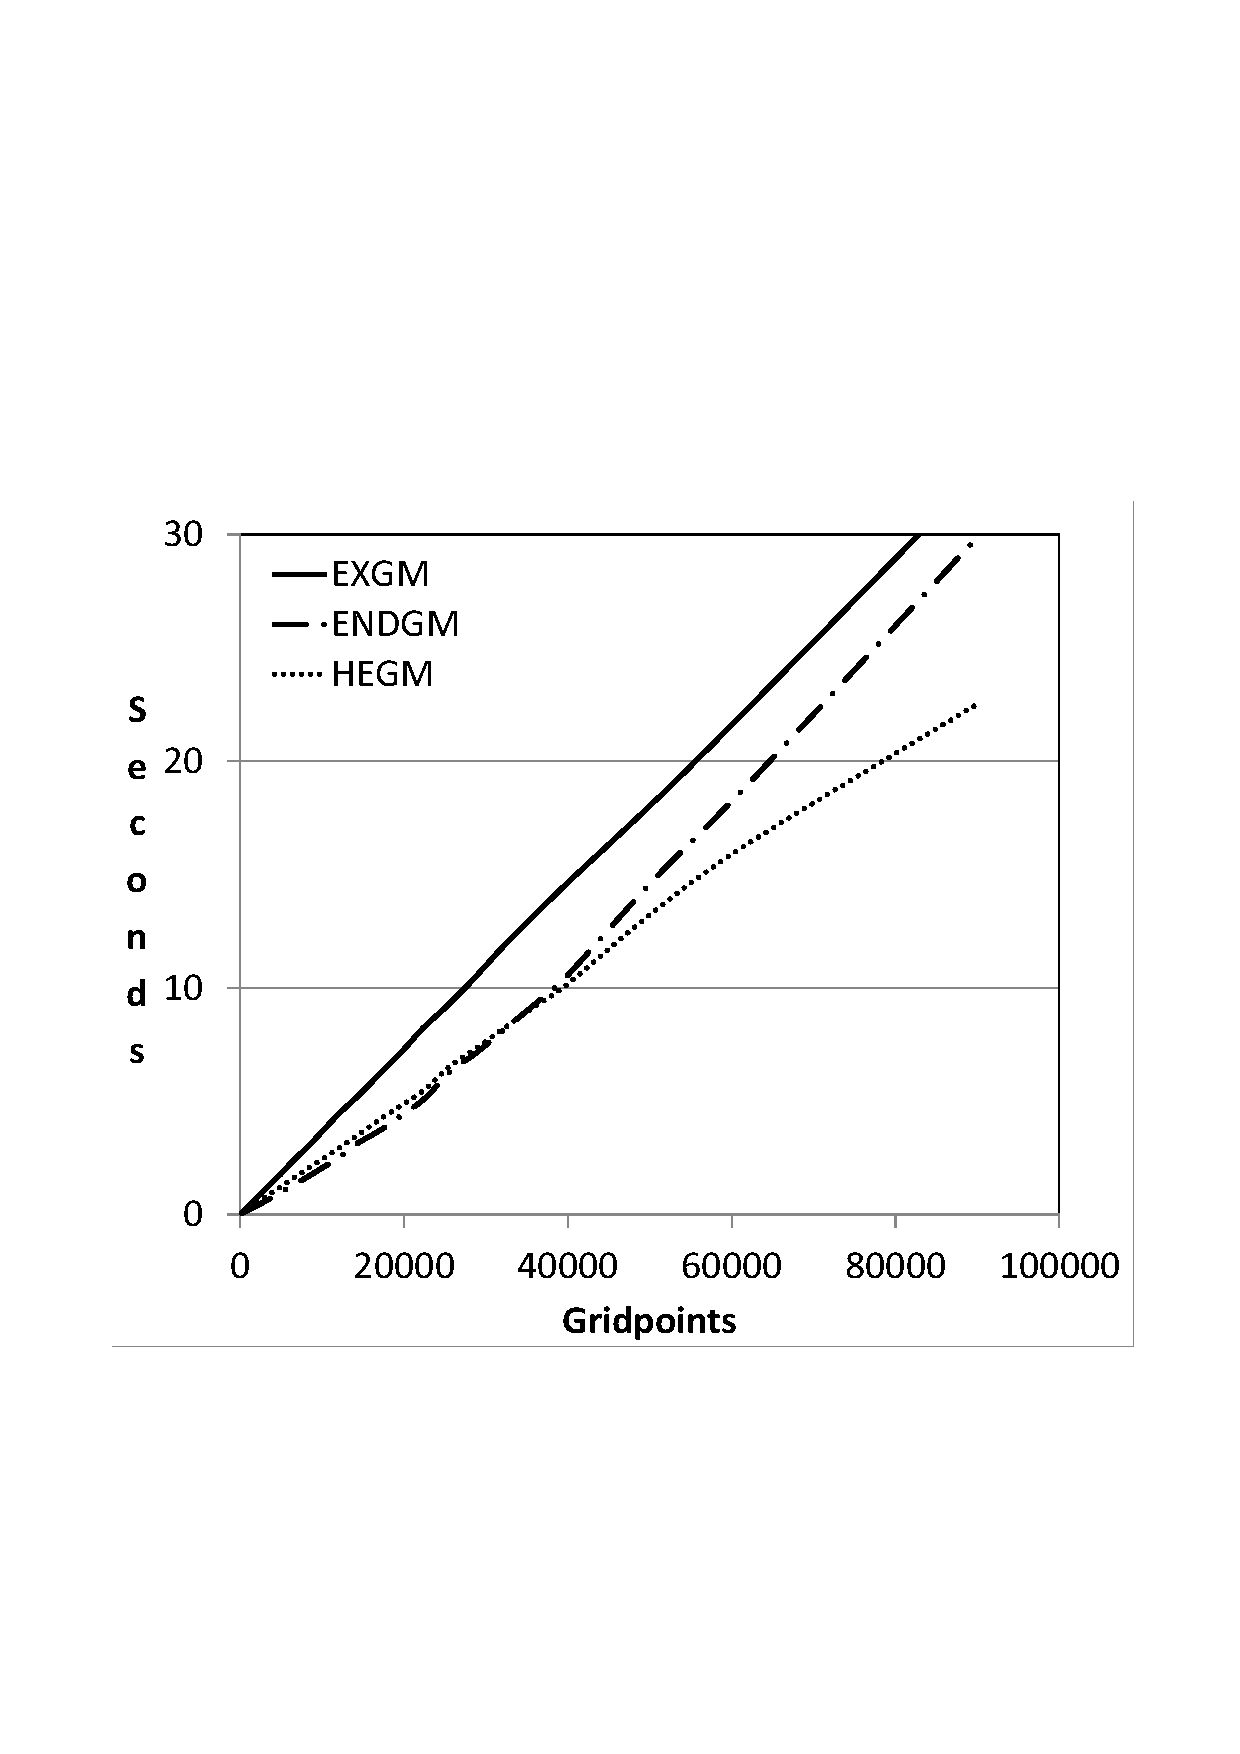
\includegraphics[height=6.0cm, width=6.0cm]{Abbildungen/Seconds_Finite.pdf}} & {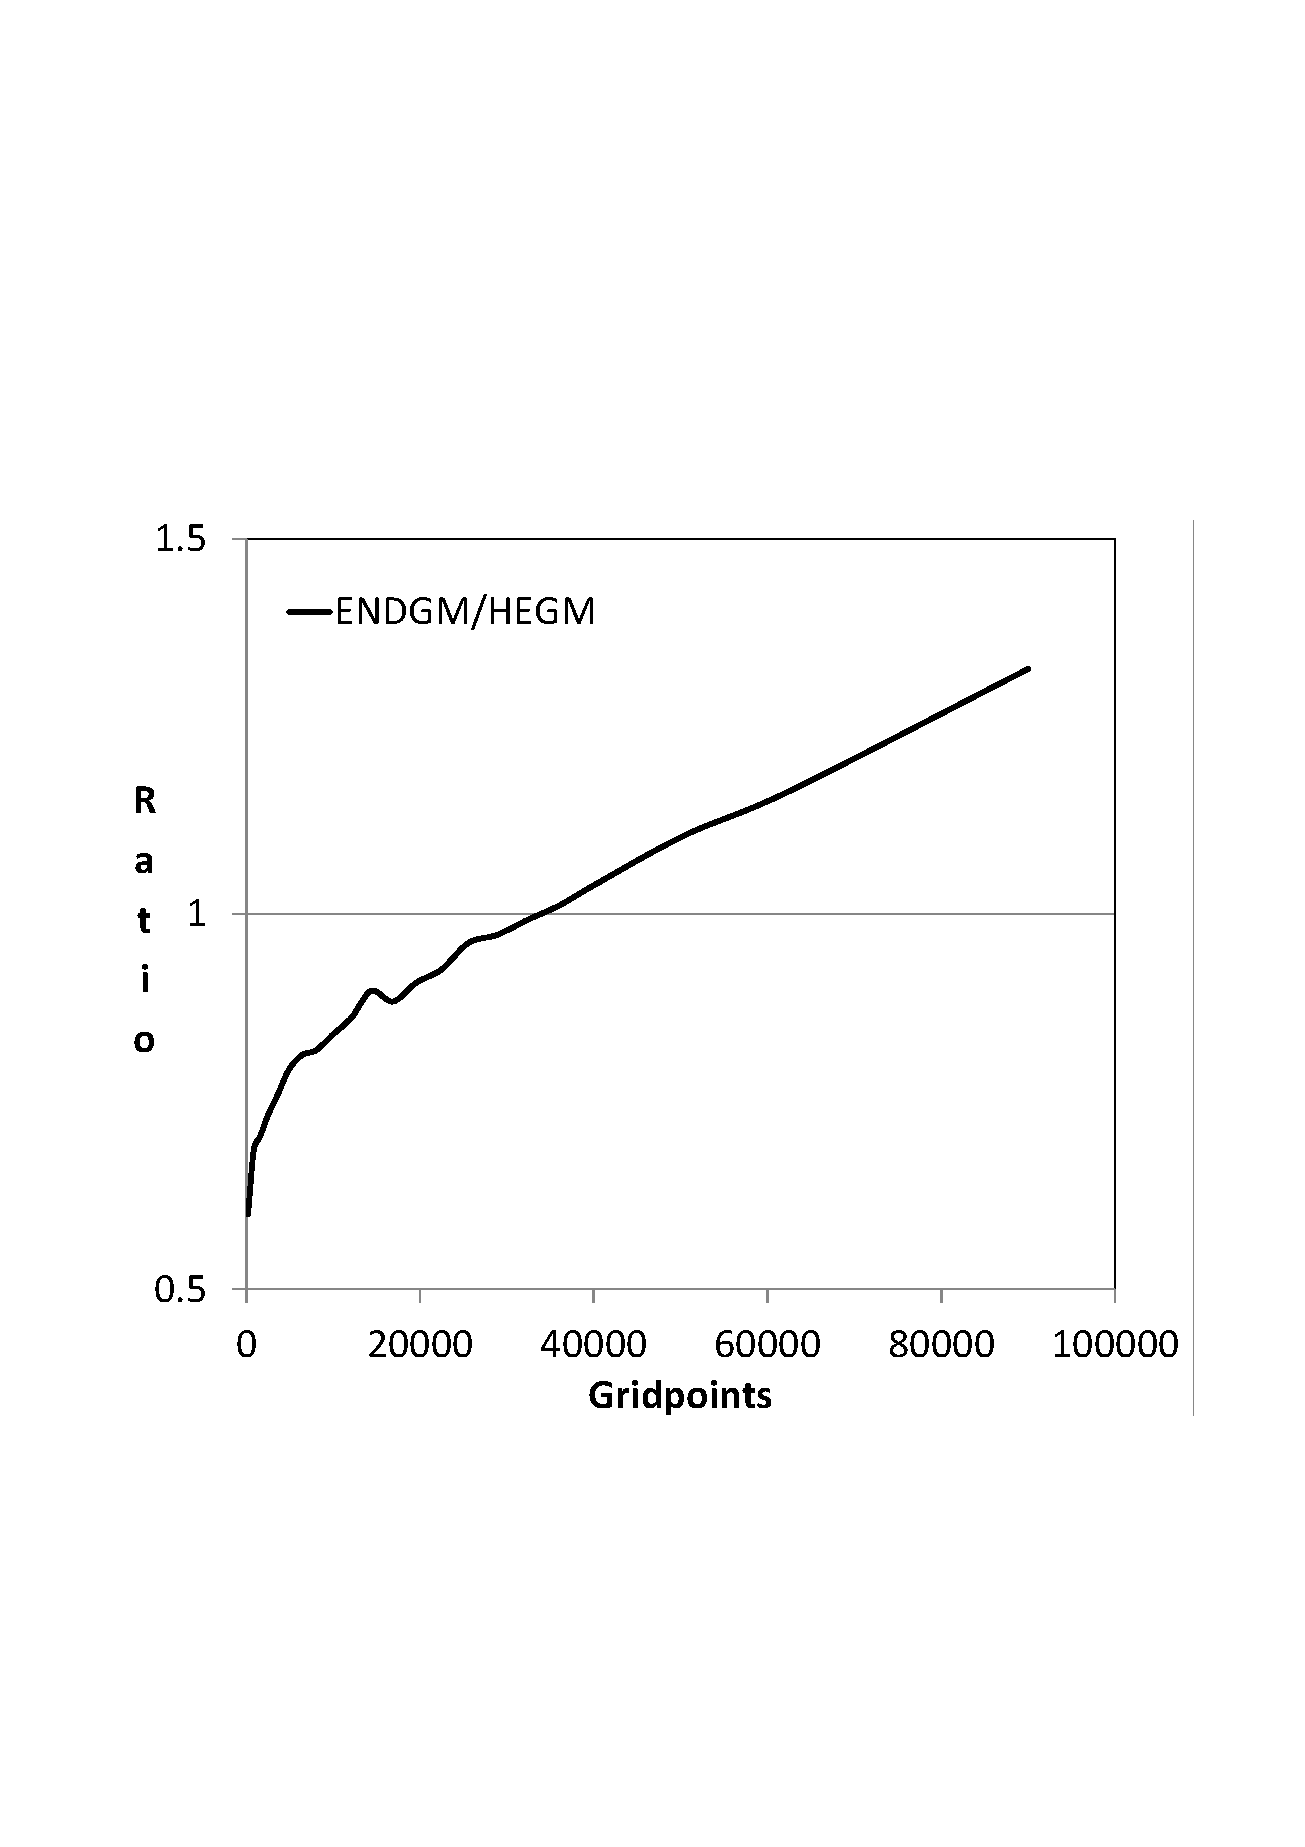
\includegraphics[height=6.0cm, width=6.0cm]{Abbildungen/Ratio_Finite.pdf}} \\
\multicolumn{2}{p{15cm}}{{\footnotesize Panel (a): Computing time as a function of grid-points in seconds (with equally many grid-points in both dimensions). Solid line: computing time of EXGM; dotted line: computing time of HEGM; dashed-dotted line: computing time of ENDGM. Panel (b): Ratio of computing time of ENDGM to HEGM as a function of grid-points (with equally many grid-points in both dimensions).}}
\end{tabular}
\label{graph_finte}
\end{figure}

\subsection{Infinite horizon}

Algorithms are also comparable in the infinite horizon setting. In all approaches, we make the same initial guesses for derivatives~$V_{0_{a}}$ and $V_{0_{h}}$ and iterate until convergence on policy functions subject to convergence criterion~$\varepsilon=10^{-6}$.\footnote{In our algorithms we define $\tilde{c}=\left\{  \left\{ \tilde{c}^{k,j}\right\}  _{k=1}^{K}\right\}  _{j=1}^{J}$ and $\tilde{\imath}=\left\{  \left\{  \tilde{\imath}^{k,j}\right\}  _{k=1}^{K}\right\}  _{j=1}^{J}$ and exit in iteration $n\,$\ if $\sup|\tilde{c}-c^{n}|\leq\varepsilon\cup|\tilde{\imath}-i^{n}|\leq\varepsilon.$}

To compute Euler equation errors we simulate the response to a shock to financial assets and health capital for 50 periods. We set the initial assets $a_{0}$ in the range if $\{250,450\}$ and health in the range of $\{50,70\}$. We compute $e_{1}$ and $e_{1}$ for the first 50 periods. Averages and maximum errors are provided in table \ref{results_infinte}.

\begin{figure}[htb] \centering
\caption{Infinite Horizon Model: Smart}
\begin{tabular}
[c]{cc}
& \\
Panel (a) & Panel (b)\\
{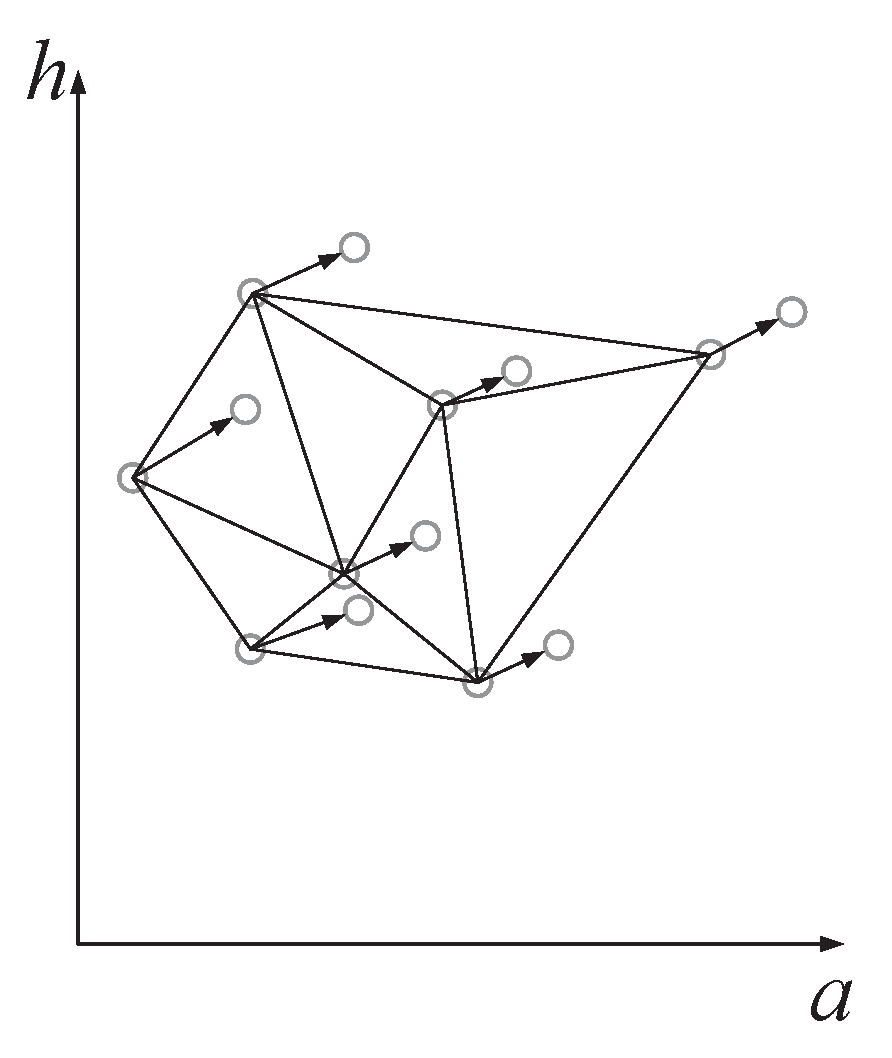
\includegraphics[height=6.0cm, width=6.0cm]{Abbildungen/Smart_1.eps}} & {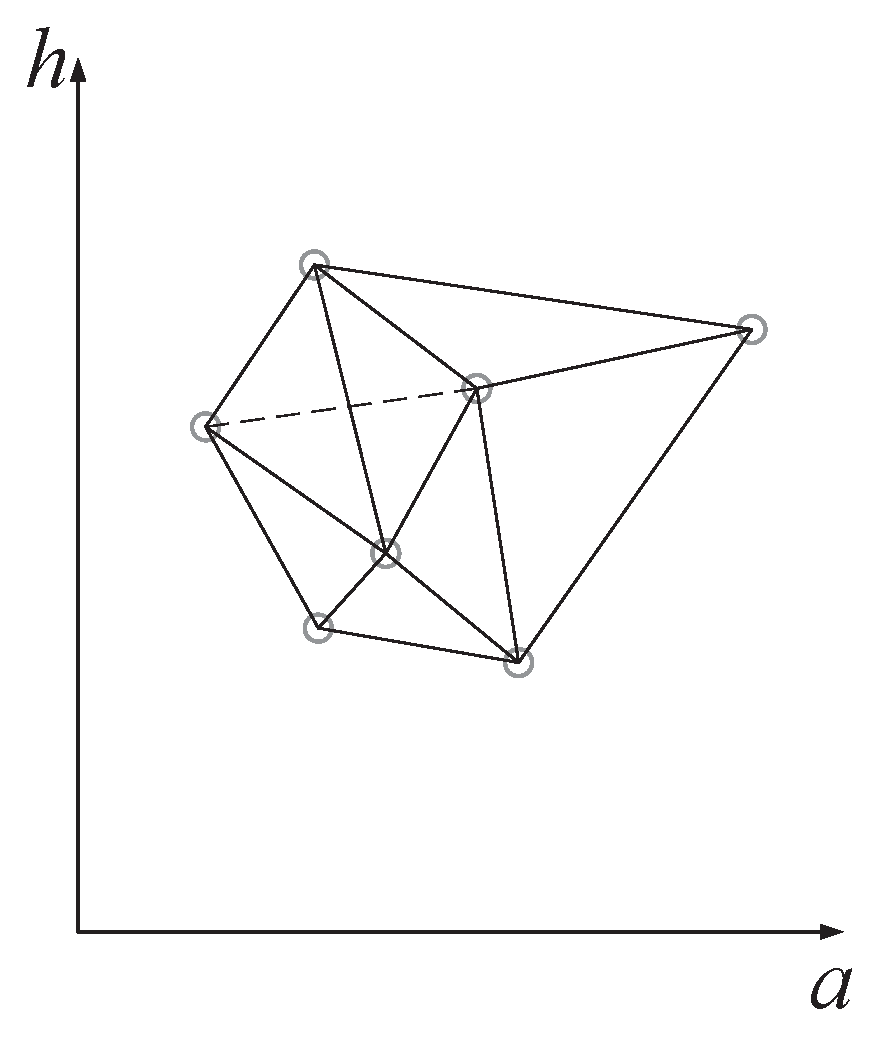
\includegraphics[height=6.0cm, width=6.0cm]{Abbildungen/Smart_2.eps}} \\
\multicolumn{2}{p{15cm}}{{\footnotesize Panel (a)  (b) ).}}
\end{tabular}
\label{graph_infinte copy(1)}
\end{figure}

As in the finite horizon setting, Euler equation errors are of similar magnitudes across algorithms---which we also achieve by appropriate settings of the respective numerical routines---so that we can again further concentrate on comparison speed only.

In the infinite horizon setting, speed of ENDGM can be increased if the Delaunay Triangulation is not constructed every iteration. Instead, we hold the triangulation pattern fixed after a certain number of iterations---$100$
in our case.\footnote{It is necessary to assure that the endogenously computed grid-points form a convex hull.} Figure \ref{graph_finte} shows the general principle. \ As in the finite horizon setting, ENDGM is the fastest method for not too many grid-points and the comparative advantage decreases for a higher number of grid-points. Both methods clearly dominate EXGM in terms of speed. Similar to our findings in the finite horizon case, for a standard choice of~$20$ to~$40$ grid-points in each dimension, ENDGM is $\frac{0.41}{0.22}\approx1.9$ to~$\frac{1.39}{0.70}\approx2.0$ times faster than HEGM and $\frac{0.69}{0.22}\approx3.1$ to~$\frac{3.03}{0.70}\approx4.3$ times faster than EXGM, cf. table \ref{results_infinte}. As in the finite horizon setting EXGM faces severe problems in terms of stability for a high number of grid-points.

\begin{figure}[htb] \centering
\caption{Infinite Horizon Model: Speed}
\begin{tabular}
[c]{cc}
& \\
Panel (a) & Panel (b)\\
{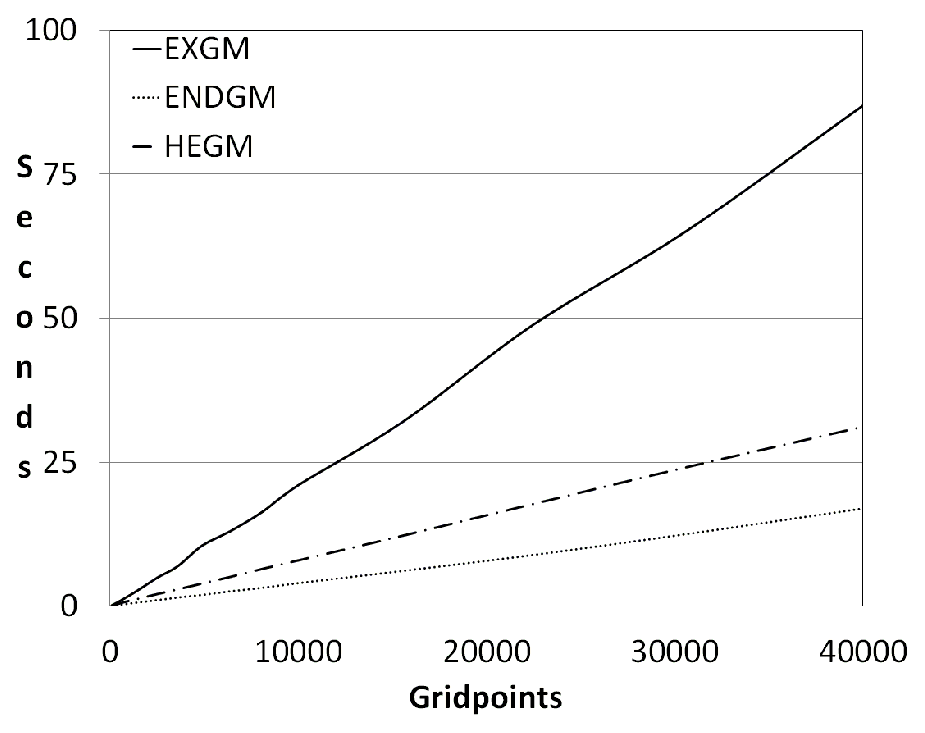
\includegraphics[height=6.0cm, width=6.0cm]{Abbildungen/speed_all_finite_smart.eps}} & {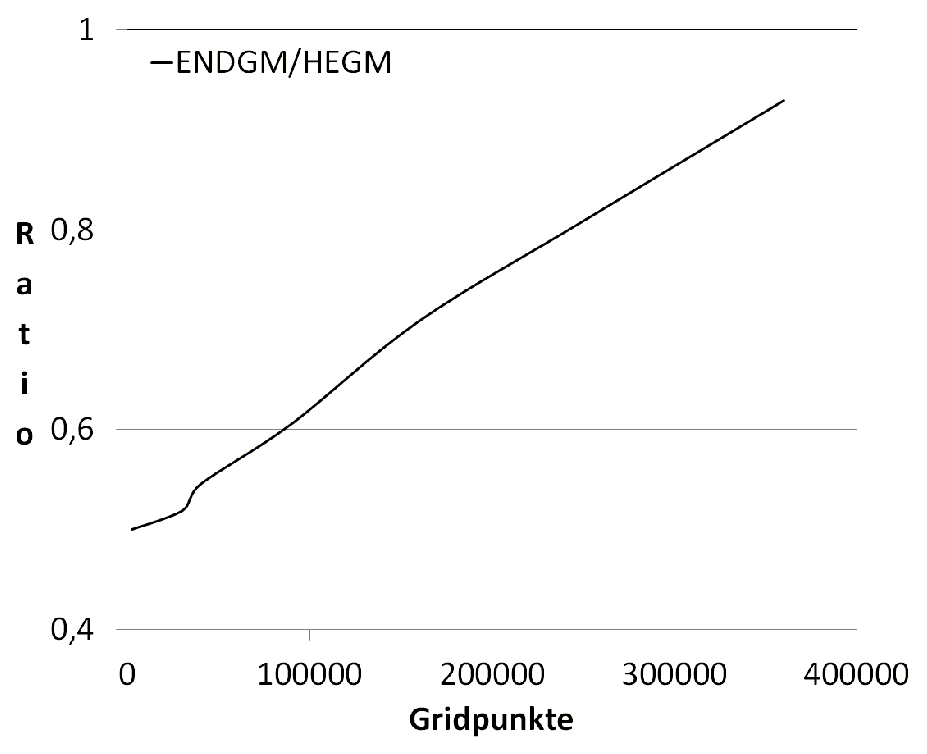
\includegraphics[height=6.0cm, width=6.0cm]{Abbildungen/rel_endgm_HEgm_infinite_smart.eps}} \\
\multicolumn{2}{p{15cm}}{{\footnotesize Panel (a) Computing time to convergence of policy functions (criterion $\varepsilon=10^{-6}$) as a function of grid-points (with equally many grid-points in both dimensions). Solid line: computing time of EXGM; dotted line: computing time of HEGM; dashed-dotted line: computing time of ENDGM. Panel (b) Ratio of computing time to convergence of ENDGM and HEGM as a function of grid-points (with equally many grid-points in both dimensions).}}
\end{tabular}
\label{graph_infinte}
\end{figure}

\begin{table}[htb] \centering
\caption{Infinite Horizon Model: Performance Results}
\begin{tabular}
[c]{p{3.5cm}||C{2cm}|C{2cm}|C{3cm}|C{3cm}}
\multicolumn{5}{p{14cm}}{}\\
& \multicolumn{2}{c|}{Speed} & \multicolumn{2}{c}{Euler error for $\left(c;i\right)$} \\ 
Number of Gridpoints for $(a,h)$ & Seconds & Relative to ENDGM & Maximum & Average \\ \hline
ENDGM &  &  &  & \\
$\left(  20,20  \right)$ &  $0.078$ &   -    & $(-2.27;\ -1.74)$ & $(-3.14;\ -2.72)$ \\
$\left(  40,40  \right)$ &  $0.296$ &   -    & $(-2.88;\ -2.25)$ & $(-3.64;\ -3.19)$ \\
$\left( 100,100 \right)$ &  $2.043$ &   -    & $(-3.59;\ -2.96)$ & $(-4.49;\ -3.95)$ \\
$\left( 200,200 \right)$ & $10.577$ &   -    & $(-4.13;\ -3.53)$ & $(-5.15;\ -4.46)$ \\
&  &  &  & \\ \hline
HEGM &  &  &  & \\
$\left(  20,20  \right)$ &  $0.234$ & $3.0$ & $(-2.27;\ -1.71)$ & $(-3.27;\ -2.85)$ \\
$\left(  40,40  \right)$ &  $0.889$ & $3.0$ & $(-3.01;\ -2.27)$ & $(-3.81;\ -3.35)$ \\
$\left( 100,100 \right)$ &  $5.538$ & $2.7$ & $(-3.62;\ -2.88)$ & $(-4.67;\ -3.93)$ \\
$\left( 200,200 \right)$ & $23.494$ & $2.2$ & $(-4.17;\ -3.56)$ & $(-5.36;\ -4.40)$ \\
&  &  &  & \\ \hline
EXGM &  &  &  & \\
$\left(  20,20  \right)$ &  $0.343$ & $4.4$ & $(-2.33;\ -1,72)$ & $(-3.33;\ -2.86)$ \\
$\left(  40,40  \right)$ &  $1.326$ & $4.5$ & $(-3.02;\ -2,28)$ & $(-3.87;\ -3.35)$ \\
$\left( 100,100 \right)$ &  $8.206$ & $4.0$ & $(-3.71;\ -2,88)$ & $(-4.67;\ -3.93)$ \\
$\left( 200,200 \right)$ & $33.291$ & $3.2$ & $(-4.20;\ -3,56)$ & $(-5.40;\ -4.40)$ \\ \hline
\multicolumn{5}{p{15cm}}{{\footnotesize Computing time to convergence of policy functions (criterion $\varepsilon=10^{-6}$) and resulting maximum and average Euler equation errors. Computing time is reported in seconds and absolute errors in units of base-10 logarithms.}}
\end{tabular}
\label{results_infinte}
\end{table}

\clearpage

\section{Conclusion}

We compare three numerical methods---the standard exogenous grid method (EXGM), Carroll's method of endogenous grid-points (ENDGM), cf. \citeN{carroll06}, and a hybrid method (HEGM)---to solve dynamic models with two continuous
state variables and occasionally binding borrowing constraints. To illustrate and to evaluate these methods we develop a life-cycle consumption-savings model with endogenous human capital formation. Evaluation of methods is based on speed and accuracy in both finite and infinite horizon settings. We show that applying the endogenous grid method in more than one dimension gives rise to irregular grids. We apply Delaunay methods to interpolate on these irregular grids. Despite this more complex interpolation, ENDGM and HEGM  clearly outperform EXGM. ENDGM dominates HEGM for small to medium sized problems (in terms of number of grid-points) whereas HEGM dominates for a large number of grid-points. For a standard choice of numbers of grid-points, ENDGM is $1.6$ to~$1.8$ times faster than HEGM.

Two additional remarks on ENDGM and HEGM are in order. First, neither of the two is a general method. Both are applicable only to specific problems at hand. This requires restrictions on the model's specification and on functional forms. Second, as HEGM uses analytical solutions in only one dimension and standard numerical methods in others, it's relative advantage decreases in the dimensionality of the problem.

In this paper, however, we restrict attention to two dimensional problems. Extensions to higher dimensions are left for future research.

\clearpage\newpage

\section{Appendix}

\label{app:equations}

To derive first-order conditions, we focus on the infinite horizon setting. As is standard in the literature, we denote next period values by symbol~$^{\prime}$.

The dynamic version of the household problem reads as
\[
V(a,h)=\underset{c,i,a^{\prime},h^{\prime}}{\max}\left\{  u(c)+\beta s\left(h^{\prime}\right)  V^{\prime}(a^{\prime},h^{\prime})\right\}
\]
subject to
\begin{align*}
a^{\prime}  &  =R\left(  a+wh-c-i\right) \\
h^{\prime}  &  =\left(  1-\delta\right)  \left(  h+f\left(  i\right)  \right) \\
a^{\prime}  &  \geq0.
\end{align*}

Assigning multiplier $\mu$ to the borrowing constraint, the two first order conditions with respect to~$c$ and~$k$ are:
\begin{equation}
\frac{\partial V\left(  a,h\right)  }{\partial c}=u_{c}-\beta s\left(h^{\prime}\right)  V_{a}^{\prime}R-R\mu\overset{!}{=}0\;\Leftrightarrow\;u_{c}-\beta s\left(  h^{\prime}\right)  RV_{a}^{\prime}=R\mu, \label{FOC1}%
\end{equation}
\begin{align}
\frac{\partial V\left(  a,h\right)  }{\partial i}  &  =s_{h}\left(  h^{\prime}\right)  \left(  1-\delta\right)  f_{i}\beta V^{\prime}+s\left(  h^{\prime}\right)  \beta\left[  V_{a}^{\prime}\left(  -R\right)  +V_{h}^{\prime}\left(1-\delta\right)  f_{i}\right]  -R\mu\overset{!}{=}0\nonumber \\
&  \Leftrightarrow s_{h}\left(  h^{\prime}\right)  \left(  1-\delta\right)f_{i}\beta V^{\prime}+s\left(  h^{\prime}\right)  \beta\left[  V_{a}^{\prime}\left(  -R\right)  +V_{h}^{\prime}\left(  1-\delta\right)  f_{i}\right] = R\mu \label{FOC2}
\end{align}

and
\begin{align*}
a^{\prime}  &  \geq0\\
\mu &  \geq0\\
a^{\prime}\mu &  =0.
\end{align*}

In order to compute optimal policies we need to distinguish two cases.

\subsection*{Case 1: Interior Solution}

In the first case the borrowing constraint is not binding so that $\mu=0$. This reduces the system of equations to%
\begin{align*}
u_{c}-\beta s\left(  h^{\prime}\right)  RV_{a}^{\prime}  &  =0 \\
s_{h}\left(  h^{\prime}\right)  \left(  1-\delta\right)  f_{i}\beta V^{\prime}+s\left(  h^{\prime}\right)  \beta\left[  V_{a}^{\prime}\left(  -R\right)+V_{h}^{\prime}\left(  1-\delta\right)  f_{i}\right]   &  =0.
\end{align*}
Rearranging gives
\begin{align*}
u_{c}  &  =\beta s\left(  h^{\prime}\right) V_{a}^{\prime}R \\
f_{i}  &  =\frac{R}{\left(  1-\delta\right)  }\frac{s\left(h^{\prime}\right)  V_{a}^{\prime}}{s_{h}\left(  h^{\prime}\right)  V^{\prime}+s\left(h^{\prime}\right)  V_{h}^{\prime}}.
\end{align*}

\subsection*{Case 2: Corner Solution---Binding Borrowing Constraint}

In the second case the borrowing constraint is binding so that $a^{\prime}=0$ and $\mu>0$. From~(\ref{FOC1}) and~(\ref{FOC2}) it then follows that
\begin{equation}
u_{c}=s_{h}\left(  h^{\prime}\right)  \beta V^{\prime}+s\left(  h^{\prime}\right)  \beta V_{h}^{\prime}\left(  1-\delta\right)  f_{i} \label{eq:uc}
\end{equation}
and
\[
u_{c}=\beta\left(  1-\delta\right)  f_{i}\left[  s_{h}\left(  h^{\prime}\right)  V^{\prime}+s\left(  h^{\prime}\right)  V_{h}^{\prime}\right]
\]
\[
a^{\prime}=0\;\Leftrightarrow\;c=a+wh-i.
\]

Making use of our assumptions on functional forms, equation~(\ref{eq:uc}) reduces in EXGM and HEGM to
\begin{align*}
& \left(  a+wh-i\right)  ^{-\theta}-\frac{1}{\left[  \left(  1-\delta\right)\left(  h+\frac{i^{1-\alpha}}{1-\alpha}\right)  \right]  ^{2}}V^{\prime}\left[  0,\left(  1-\delta\right)  \left(  h+\frac{i^{1-\alpha}}{1-\alpha}\right)  \right]  \beta\left(  1-\delta\right)  i^{-\alpha} \\
&  -\left[  1-\frac{1}{\left[  \left(  1-\delta\right)  \left(  h+\frac{i^{1-\alpha}}{1-\alpha}\right)  \right]  }\right]  \left[  V_{h}^{\prime}\left[  0,\left(  1-\delta\right)  \left(  h+\frac{i^{1-\alpha}}{1-\alpha}\right)  \right]  \right]  \beta\left(  1-\delta\right)  i^{-\alpha}=0
\end{align*}
and in ENDGM to
\begin{align*}
&  \left(  a+w\frac{h^{\prime}}{1-\delta}-i^{\alpha}-i\right)  ^{-\theta}-\frac{1}{\left[  h^{\prime}\right]  ^{2}}\beta V^{\prime}\left[0,h^{\prime}\right]  \left(  1-\delta\right)  i^{-\alpha}\\
&  -\left[  1-\frac{1}{1+h^{\prime}}\right]  \beta\left[  V_{h}^{\prime}\left[  0,h^{\prime}\right]  \right]  \left(  1-\delta\right)  i^{-\alpha}=0.
\end{align*}
Observe that this equation is not linear in $i$. We therefore need to use a numerical routine in the region where the borrowing constraint is binding also for ENDGM, cf. our discussion in the main text in Subsection~\ref{ss:analendgm}.

\qquad

In both cases---i.e. for interior solutions and for binding borrowing constraints---the envelope conditions are
\begin{align*}
\frac{\partial V\left(  x,h\right)  }{\partial a}  &  \equiv V_{a}=\beta V_{a}^{\prime}R+R\mu=u_{c}\\
\frac{\partial V\left(  x,h\right)  }{\partial h}  &  \equiv V_{h}\\
&  =\beta s_{h}\left(  h^{\prime}\right)  V(a^{\prime},h^{\prime})\left(1-\delta\right)  +\beta s\left(  h^{\prime}\right)  V_{a}(a^{\prime},h^{\prime})wR+\beta s\left(  h^{\prime}\right)  V_{h}(a^{\prime},h^{\prime})\left(  1-\delta\right)  +R\mu \\
&  =\left(  w+\frac{1}{f_{i}}\right) u_{c}.
\end{align*}
\newpage
\bibliographystyle{chicago}
\bibliography{comparison}

\end{document}